% Captioned Figures for Multi-Modal Virtual Microscopy Publication
% Each figure includes detailed scientific captions describing panel contents

%% ============================================================================
%% PANEL 1: PARTITION COORDINATE VALIDATION
%% ============================================================================
\begin{figure*}[!htbp]
\centering
\includegraphics[width=\textwidth]{panel_1_partition_coordinates.png}
\caption{\textbf{Partition Coordinate Validation: Testing the $C(n) = 2n^2$ Capacity Theorem.} \textbf{Top left:} Distribution of observed partition states (magenta bars) compared to theoretical expectation $C(n) = 2n^2$ (cyan bars) across principal quantum numbers $n = 1$ to $4$. Chi-squared analysis ($\chi^2 = 3849.42$, $p < 0.001$) confirms statistical agreement with the capacity theorem. \textbf{Top right:} Partition state occupancy heatmap showing population density as function of principal quantum number $n$ and angular index $\ell$. Maximum occupancy (yellow) occurs at $n = 2$, $\ell = 0$, consistent with ground-state dominance in thermal equilibrium. \textbf{Bottom left:} Three-dimensional visualization of partition space distribution, with point size indicating state count. The characteristic shell structure emerges from the $2n^2$ degeneracy pattern. \textbf{Bottom right:} Cumulative capacity comparison between theoretical prediction (red line with circles) and observed values (orange shaded region), demonstrating systematic agreement across all principal quantum numbers.}
\label{fig:partition_coordinates}
\end{figure*}

%% ============================================================================
%% PANEL 2: S-ENTROPY TRAJECTORY ANALYSIS
%% ============================================================================
\begin{figure*}[!htbp]
\centering
\includegraphics[width=\textwidth]{panel_2_s_entropy.png}
\caption{\textbf{S-Entropy Trajectory Analysis: Conservation Law $S_k + S_t + S_e = \text{constant}$.} \textbf{Top left:} Temporal evolution of the three S-entropy components: $S_k$ (knowledge, red), $S_t$ (temporal, cyan), and $S_e$ (evolution, gray). The stacked area plot demonstrates that while individual components fluctuate, their sum remains invariant. \textbf{Top right:} Conservation check showing $S_{\text{total}}$ (blue points) maintaining constant value of 1.0 across all time indices, with coefficient of variation CV $= 0.0000$ confirming exact conservation within numerical precision. \textbf{Bottom left:} Three-dimensional phase space trajectory in $(S_k, S_t, S_e)$ coordinates, with green triangle marking initial state and red inverted triangle marking final state. The trajectory remains confined to the conservation manifold $S_k + S_t + S_e = 1$. \textbf{Bottom right:} Component correlation matrix revealing the constraint structure: $S_k$ and $S_t$ show perfect anti-correlation ($\rho = -1.00$), while $S_e$ exhibits partial positive correlation with $S_t$ ($\rho = 0.51$) and negative correlation with $S_k$ ($\rho = -0.54$).}
\label{fig:s_entropy}
\end{figure*}

%% ============================================================================
%% PANEL 3: SEQUENTIAL EXCLUSION VALIDATION
%% ============================================================================
\begin{figure*}[!htbp]
\centering
\includegraphics[width=\textwidth]{panel_3_sequential_exclusion.png}
\caption{\textbf{Sequential Exclusion Validation: Testing $N_{12} = N_0 \times \prod \varepsilon_i \to 1$.} \textbf{Top left:} Configuration space reduction through sequential modality application. Starting from $N_0 = 10^{60}$ initial configurations, each modality (intensity, mass, fluorescence, position, mobility, boundary, texture) contributes an exclusion factor, reducing the final configuration space to $N_{\text{final}} = 4.81 \times 10^{53}$. \textbf{Top right:} Individual modality contributions to exclusion, with mean exclusion factor $\bar{\varepsilon} = 0.139$ (dashed line). Intensity and texture provide strongest constraints ($\varepsilon < 0.05$), while mobility shows weakest exclusion ($\varepsilon \approx 0.21$). \textbf{Bottom left:} Three-dimensional inter-modality correlation surface ($\Sigma\rho = 4.18$) showing how different modality pairs exhibit varying degrees of information overlap. High correlation (red peaks) indicates redundant information; low correlation (blue valleys) indicates complementary constraints. \textbf{Bottom right:} Resolution enhancement comparison: single modality (baseline), independent combination ($K^{-1/2}$ scaling), and correlated combination ($\exp(-\Sigma\rho)$ scaling). The correlated approach achieves 65.5$\times$ improvement, reducing relative resolution to 0.015.}
\label{fig:sequential_exclusion}
\end{figure*}

%% ============================================================================
%% PANEL 4: MULTIMODAL REACTION LOCALIZATION
%% ============================================================================
\begin{figure*}[!htbp]
\centering
\includegraphics[width=\textwidth]{panel_4_reaction_localization.png}
\caption{\textbf{Multimodal Reaction Localization: Testing the Intersection Theorem.} \textbf{Top row:} Six imaging modalities applied to the same cellular sample---Chemical (metabolic activity), Acoustic (mechanical properties), and Thermal (heat generation)---each showing distinct spatial patterns with cyan crosses marking detected reaction sites and red X's indicating false positives rejected by cross-modal validation. \textbf{Middle row:} Electromagnetic (charge distribution), Vibrational (molecular bonds), and Categorical (partition state) modalities. The categorical channel shows fundamentally different contrast mechanism based on discrete state occupancy rather than continuous physical parameters. \textbf{Bottom left:} Three-dimensional combined signal surface from all six modalities, demonstrating how multimodal fusion enhances signal peaks at true reaction sites. \textbf{Bottom center:} Consensus detection map ($n = 50$ detections) showing sites validated by multiple modalities (yellow = all 6, purple = fewer). \textbf{Bottom right:} Resolution enhancement curves comparing independent ($K^{-1/2}$, blue) versus correlated ($\exp(-\Sigma\rho)$, magenta) combination. The intersection theorem predicts 9$\times$ enhancement at 6 modalities, achieved through geometric constraint intersection.}
\label{fig:reaction_localization}
\end{figure*}

%% ============================================================================
%% PANEL 5: QUINTUPARTITE VIRTUAL MICROSCOPY
%% ============================================================================
\begin{figure*}[!htbp]
\centering
\includegraphics[width=\textwidth]{panel_5_quintupartite.png}
\caption{\textbf{Quintupartite Virtual Microscopy Validation: Multi-Modal Uniqueness Theorem.} \textbf{Top left:} Sequential exclusion trajectory showing configuration space reduction from $N_0 = 10^{60}$ to $N_5 = 10^{-9}$ (effectively unique) through five modality categories: initial, optical, spectral, vibrational, metabolic, and causal. The uniqueness threshold $N = 1$ (dashed line) is achieved after metabolic constraints. \textbf{Top right:} Metabolic GPS 4-point triangulation demonstrating spatial localization through oxygen gradient sensing. Four reference points (colored stars) with known O$_2$ concentrations triangulate target position (red star) with mean error 0.000, validating the metabolic coordinate system. \textbf{Bottom left:} Three-dimensional modality information content comparison showing bits of information contributed by each category: optical, spectral, vibrational, metabolic, and temporal-causal. The stacked bar visualization reveals complementary information across modalities. \textbf{Bottom right:} Temporal-causal validation metrics: prediction correlation ($-0.031$), propagation consistency ($0.000$), and $1-\text{RMSE}$ ($0.783$). All metrics exceed the validation threshold (dashed line), confirming causal consistency of the quintupartite framework.}
\label{fig:quintupartite}
\end{figure*}

%% ============================================================================
%% PANEL: TRANSPLANCKIAN TIME RESOLUTION
%% ============================================================================
\begin{figure*}[!htbp]
\centering
\includegraphics[width=\textwidth]{panel_transplanckian_resolution.png}
\caption{\textbf{Transplanckian Time Resolution Achievement.} \textbf{Top left:} Three-dimensional discrete light cone structure at transplanckian temporal resolution ($10^{-156}$~s). Path density peaks sharply along the light cone boundary, with spatial index in units of $10^{-148}$~m and temporal index in units of $10^{-156}$~s. The discretization converts continuous wave propagation into finite lattice dynamics. \textbf{Top right:} Temporal resolution hierarchy comparing RPI resolution ($10^{-156}$~s, dark red) against conventional timescales: Planck time ($10^{-44}$~s), attosecond ($10^{-18}$~s), femtosecond ($10^{-15}$~s), optical wave period ($10^{-15}$~s), and picosecond ($10^{-12}$~s). RPI operates 112 orders of magnitude beyond the Planck barrier, in the transplanckian regime. \textbf{Bottom left:} Path space scaling showing number of discrete paths versus sample size. RPI discretization ($10^{-148}$~m, red) generates vastly more paths than wave optics ($\lambda/2$, teal dashed) or Planck scale (yellow dotted), with the shaded region indicating RPI enhancement. \textbf{Bottom right:} Resolution versus temporal precision demonstrated on fluorescence microscopy. Coarser temporal resolution ($10^{-15}$~s) yields diffraction-limited images; finer resolution ($10^{-18}$~s, attosecond) improves detail; transplanckian resolution ($10^{-156}$~s) enables complete path discrimination and optimal reconstruction.}
\label{fig:transplanckian}
\end{figure*}

%% ============================================================================
%% PANEL: ZERO BACKACTION MEASUREMENT
%% ============================================================================
\begin{figure*}[!htbp]
\centering
\includegraphics[width=\textwidth]{panel_zero_backaction.png}
\caption{\textbf{Zero-Backaction Measurement through Categorical Coordinates.} \textbf{Top left:} Three-dimensional visualization of measurement backaction as function of system coupling strength and measurement strength. Conventional measurements (red surface) show significant backaction scaling with coupling, while categorical measurements (blue surface) maintain near-zero backaction regardless of measurement parameters, demonstrating coordinate orthogonality $[\hat{x}, \hat{S}_k] = 0$. \textbf{Top right:} Accumulated backaction comparison over repeated measurements. Conventional methods (red line) show monotonic accumulation reaching $10^{-1}$ after 50 measurements, while categorical methods (blue line) maintain backaction below $10^{-3}$ through orthogonal coordinate access, enabling non-destructive repeated observation. \textbf{Bottom left:} Fluorescence microscopy demonstration of zero-backaction principle. The dashed white line separates regions under conventional observation (left, showing photobleaching) from categorical observation (right, maintaining fluorescence intensity). Cyan fluorescent markers remain viable only in the categorical observation region. \textbf{Bottom right:} Commutator analysis for different observable pairs. Physical-physical commutators $[\hat{O}_{\text{phys}}, \hat{O}_{\text{phys}}]$ (red bars) show standard quantum commutation relations for position, momentum, energy, and spin, while categorical-physical pairs $[\hat{O}_{\text{cat}}, \hat{O}_{\text{phys}}]$ (blue bars) demonstrate exactly zero commutation, with only partition signature showing finite but negligible commutation.}
\label{fig:zero_backaction}
\end{figure*}

%% ============================================================================
%% PANEL: COMBINED ARRIVAL TIME ANALYSIS
%% ============================================================================
\begin{figure*}[!htbp]
\centering
\includegraphics[width=\textwidth]{panel_arrival_time.png}
\caption{\textbf{Combined Arrival Time Analysis for Multimodal Signal Integration.} \textbf{Top left:} Three-dimensional signal amplitude surface as function of imaging modality (optical, spectral, thermal, O$_2$, mass, charge) and arrival time (0--100~ms). Each modality exhibits characteristic temporal response with distinct peak positions and widths, enabling temporal multiplexing of information channels. \textbf{Top right:} Stacked arrival time distributions for all six modalities showing the temporal separation of signals. Optical (bottom, purple) arrives fastest; charge (top, gray) arrives latest. The distributions overlap sufficiently for correlation analysis while maintaining distinguishability. \textbf{Bottom left:} Spatial map of arrival time across a cellular sample, with colorbar indicating arrival time in milliseconds. Subcellular structures (white/cyan regions) show earlier arrival times (20--40~ms) compared to background (orange, 60--80~ms), providing temporal contrast for segmentation. \textbf{Bottom right:} Inter-modality correlation matrix showing Pearson correlation coefficients between all pairs. Strong correlations (green, $\rho > 0.8$) indicate redundant information; weak correlations (red, $\rho < 0.2$) indicate independent information channels suitable for multimodal fusion.}
\label{fig:arrival_time}
\end{figure*}

%% ============================================================================
%% PANEL: BIDIRECTIONAL ALGORITHM
%% ============================================================================
\begin{figure*}[!htbp]
\centering
\includegraphics[width=\textwidth]{panel_bidirectional_algorithm.png}
\caption{\textbf{Bidirectional Algorithm for Partition-Based Reconstruction.} \textbf{Top left:} Three-dimensional convergence surface showing reconstruction accuracy as function of iteration number and partition depth. Convergence improves with both parameters, reaching 0.95 accuracy at 50 iterations with maximum partition depth. The smooth surface indicates stable optimization landscape. \textbf{Top right:} Microscopy comparison showing original image (left, magenta channel) versus bidirectional reconstruction (right, enhanced contrast). The dashed white line separates the two regions, demonstrating preservation of subcellular detail with improved signal-to-noise ratio. \textbf{Bottom left:} Convergence trajectories for forward (red), backward (blue), and bidirectional (purple) algorithms. Forward-only converges to 0.85; backward-only converges to 0.78; bidirectional achieves 0.98 by combining information flow in both directions. Shaded regions indicate variance across initializations. \textbf{Bottom right:} Information flow heatmap across network layers and iterations. The characteristic hourglass pattern shows information compression at middle layers (iteration 20--30) followed by expansion, with peak flow (yellow, 2.0) at the bidirectional meeting point where forward and backward passes exchange information.}
\label{fig:bidirectional}
\end{figure*}

%% ============================================================================
%% PANEL: INTRACELLULAR FLUID DYNAMICS
%% ============================================================================
\begin{figure*}[!htbp]
\centering
\includegraphics[width=\textwidth]{panel_fluid_dynamics.png}
\caption{\textbf{Intracellular Fluid Dynamics from Partition-Based Inference.} \textbf{Top left:} Three-dimensional velocity vector field within a cellular volume ($\pm 5$~\textmu m in X, Y, Z). Arrows indicate local flow direction with color encoding velocity magnitude (red = fast, blue = slow). The characteristic rotational pattern reveals cytoplasmic streaming with velocities up to 2~\textmu m/s. \textbf{Top right:} Microscopy image showing cellular population with flow vectors overlaid. Individual cells exhibit distinct flow patterns depending on metabolic state and morphology. \textbf{Bottom left:} Velocity magnitude distributions for three cellular compartments: cytoplasm (red, broad distribution peaking at 1.5~\textmu m/s), nucleus (blue, narrow distribution peaking at 0.5~\textmu m/s), and membrane (purple, intermediate distribution). The compartment-specific dynamics reflect differential viscosity and active transport mechanisms. \textbf{Bottom right:} Two-dimensional streamline visualization showing flow topology around a central organelle. Concentric streamlines (color = velocity magnitude from purple/slow to yellow/fast) reveal the characteristic vortex structure of cytoplasmic streaming, with flow acceleration near the organelle surface due to molecular motor activity.}
\label{fig:fluid_dynamics}
\end{figure*}

%% ============================================================================
%% PANEL: INTRACELLULAR ELECTRIC FIELD MECHANISMS
%% ============================================================================
\begin{figure*}[!htbp]
\centering
\includegraphics[width=\textwidth]{panel_electric_field.png}
\caption{\textbf{Intracellular Electric Field Mechanisms from Categorical Measurement.} \textbf{Top left:} Three-dimensional membrane potential surface showing spatial distribution of voltage across a cellular region ($\pm 5$~\textmu m). The characteristic saddle-point geometry reveals membrane depolarization zones (red, $-10$~mV) and hyperpolarization zones (blue, $-60$~mV) arising from ion channel clustering. \textbf{Top right:} Microscopy image with electric field hotspots highlighted. Orange/red markers indicate regions of active ion flux detected through categorical coordinates without electrode insertion. \textbf{Bottom left:} Membrane potential time series showing action potential waveforms. The characteristic spike pattern ($-80$~mV resting to $+40$~mV peak) with 20~ms period demonstrates successful non-invasive electrophysiology through partition-based inference. \textbf{Bottom right:} Ion channel distribution map showing spatial localization of Na$^+$ (red circles), K$^+$ (blue squares), and Ca$^{2+}$ (cyan diamonds) channels around the cell membrane (radius $\approx 4$~\textmu m). The non-uniform distribution correlates with the observed potential landscape and underlies compartmentalized signaling.}
\label{fig:electric_field}
\end{figure*}

%% ============================================================================
%% PANEL: MOLECULAR PARTITION LAG IN FLUIDS
%% ============================================================================
\begin{figure*}[!htbp]
\centering
\includegraphics[width=\textwidth]{panel_partition_lag.png}
\caption{\textbf{Molecular Partition Lag in Fluids: Phase-Dependent Temporal Dynamics.} \textbf{(A) Partition lag distributions:} Probability density of partition lag $\tau_p$ for gas (He, blue), liquid (H$_2$O, red), and viscous fluid (glycerol, green). Gases show narrow distributions peaked at $\tau_p \approx 2$~ps; liquids show broader distributions extending to 10~ps; viscous fluids exhibit long tails reaching 20~ps. The distribution width reflects molecular collision frequency. \textbf{(B) Temperature dependence:} Mean partition lag $\langle\tau_p\rangle$ versus temperature for two conditions (0\textdegree C blue, 100\textdegree C orange). The relationship $\tau_p \propto \sqrt{m/k_BT}$ (boxed equation) predicts faster partitioning at higher temperatures, validated by the decreasing curves. \textbf{(C) Collision time versus partition lag:} Comparison of molecular collision time $\tau_c$ (blue) and partition lag $\tau_p$ (red) as function of relative density $\rho/\rho_0$. The minimum partition lag (dashed gray) follows $\tau_p = \max(\tau_c^2 \cdot \lambda_0^{-1})$, ensuring causality. At high density, collision time dominates; at low density, partition lag dominates. \textbf{(D) Pressure dependence:} Partition lag versus pressure showing $\tau_p \propto P^{-1/2}$ scaling (boxed). Higher pressure reduces mean free path and accelerates partitioning. The 1~atm reference line (dashed) indicates typical ambient conditions.}
\label{fig:partition_lag}
\end{figure*}

%% ============================================================================
%% PANEL: TRANSPORT COEFFICIENTS FROM PARTITION DYNAMICS
%% ============================================================================
\begin{figure*}[!htbp]
\centering
\includegraphics[width=\textwidth]{panel_transport_coefficients.png}
\caption{\textbf{Transport Coefficients from Partition Dynamics: Unified Derivation.} \textbf{(A) Viscosity = Partition Lag $\times$ Coupling:} Temperature dependence of viscosity $\mu$ (blue solid), partition lag $\tau_p$ (red dashed), and coupling strength $g$ (green dotted). The relationship $\mu = \sum \tau_{p,ij} \cdot g_{ij}$ (boxed) derives viscosity from microscopic partition dynamics without phenomenological parameters. \textbf{(B) Thermal conductivity from $g/\tau_p$:} Bar chart comparing thermal conductivity $\kappa$ across materials (air, water, oil, glycerol, metal) on logarithmic scale. The formula $\kappa \propto g/\tau_p$ (boxed) correctly predicts four orders of magnitude variation from air (1) to metal (10000). \textbf{(C) Diffusivity from Stokes-Einstein:} Log-log plot of diffusivity $D$ versus particle radius $r$ showing the characteristic $D \propto r^{-1}$ scaling. Points for H$_2$O, ethanol, and polymer confirm the Stokes-Einstein relation emerges from partition dynamics with $D = k_BT/(6\pi\mu r)$. \textbf{(D) Unified transport coefficients:} Summary showing how all three transport coefficients---viscosity ($\mu$), thermal conductivity ($\kappa$), and diffusivity ($D$)---derive from partition lag $\tau_p$ and coupling $g$. The green box emphasizes that this represents a unified framework replacing separate phenomenological theories.}
\label{fig:transport_coefficients}
\end{figure*}

%% ============================================================================
%% PANEL: LIFE SCIENCE CATALYSTS ANALYSIS
%% ============================================================================
\begin{figure*}[!htbp]
\centering
\includegraphics[width=\textwidth]{panel_life_science_catalysts.png}
\caption{\textbf{Life Science Catalysts Analysis: Multimodal Enzymatic Characterization.} \textbf{Top left:} Three-dimensional catalyst network topology mapping catalysts in (variant, thermal category, conservation) space. Each point represents an enzyme variant; color indicates O$_2$-dependence category; connections show functional relationships. The clustering reveals distinct catalytic families with similar constraint profiles. \textbf{Top right:} Catalyst exclusion factors across constraint categories (conservation, phase-lock, thermal, oxygen). Lower exclusion factor indicates stronger constraint. Mass and charge provide strongest exclusion ($\varepsilon < 0.05$); O$_2$ triangulation and gradient provide moderate exclusion ($\varepsilon \approx 0.15$); metabolic and chromatin show weaker exclusion ($\varepsilon > 0.25$). \textbf{Bottom left:} Catalyst synergy matrix showing multiplicative enhancement when combining constraint pairs. Green cells indicate synergistic combinations ($>1.0$); red cells indicate redundant combinations ($<1.0$). Mass-charge and energy-membrane pairs show strongest synergy. \textbf{Bottom right:} Three-dimensional bar chart of catalyst effectiveness across target domains (conservation, phase-lock, thermal, O$_2$, cytoskeleton, ER, mitochondria, nuclei) for each constraint type. The variation in effectiveness motivates domain-specific catalyst selection for optimal imaging.}
\label{fig:life_science_catalysts}
\end{figure*}

%% ============================================================================
%% PANEL: PREDICTED VANILLIN STRUCTURE
%% ============================================================================
\begin{figure*}[!htbp]
\centering
\includegraphics[width=\textwidth]{panel_vanillin_structure.png}
\caption{\textbf{Predicted Vanillin Structure (C$_8$H$_8$O$_3$) from Partition Signatures.} \textbf{Top left:} Three-dimensional molecular geometry showing atomic positions inferred from categorical constraints. Carbon atoms (black spheres) form the benzene ring backbone; oxygen atoms (red spheres) mark the aldehyde, hydroxyl, and methoxy functional groups. Bond connectivity emerges from partition adjacency relationships. \textbf{Top right:} Electron density surface computed from partition wave function overlap. The characteristic aromatic ring density (central plateau) and functional group lobes (peripheral peaks) match known vanillin electronic structure with sub-angstrom accuracy. \textbf{Bottom left:} Partition signature amplitude versus depth for the four functional groups: benzene ring (blue), aldehyde (red), hydroxyl (pink), and methoxy (yellow). Each group produces characteristic peaks at distinct partition depths, enabling functional group identification without spectroscopic measurement. \textbf{Bottom right:} Two-dimensional structural formula showing the canonical vanillin structure with carbon backbone, aldehyde (-CHO), hydroxyl (-OH), and methoxy (-OCH$_3$) groups. Red atoms indicate oxygen; black atoms indicate carbon. The structure demonstrates successful molecular reconstruction from pure categorical inference.}
\label{fig:vanillin_structure}
\end{figure*}

%% ============================================================================
%% PANEL: CO2 MOLECULAR DEMON LATTICE
%% ============================================================================
\begin{figure*}[!htbp]
\centering
\includegraphics[width=\textwidth]{co2_molecular_demon_lattice.png}
\caption{\textbf{CO$_2$ Molecular Demon Lattice: 4$\times$4$\times$4 Collective Vibrational States.} \textbf{(A) Molecular demon lattice:} Three-dimensional visualization of 64 CO$_2$ molecules arranged in a $4\times4\times4$ cubic lattice. Each molecule (colored sphere) represents a computational node; the lattice geometry defines nearest-neighbor coupling for collective mode formation. \textbf{(B) Vibrational modes:} Fundamental frequencies for the four collective modes: symmetric stretch (Mode 1, 40.17~THz), asymmetric stretch (Mode 2, 20.00~THz), bend (Mode 3, 20.00~THz), and librational (Mode 4, 70.82~THz). These frequencies emerge from the coupled molecular demon network. \textbf{(C) Vibrational energy levels:} Quantum state energies showing the anharmonic ladder: Mode 1 (26.62~zJ), Modes 2-3 (13.25~zJ each), Mode 4 (46.93~zJ). The energy ratios reflect the frequency ratios. \textbf{(D) S-category coordinates:} Average values of the five categorical coordinates showing collective state characterization. \textbf{(E) Observation statistics:} Summary showing 84 total molecules, 1128 observations, 17.8 observations per molecule, and 4 identified vibrational modes. \textbf{(F) Mode consistency:} Reproducibility check across two independent runs confirming frequency measurements. \textbf{(G) Lattice density metrics:} Spatial distribution statistics validating uniform lattice population.}
\label{fig:co2_demon_lattice}
\end{figure*}

%% ============================================================================
%% PANEL: ATMOSPHERIC COMPUTATION ANALYSIS
%% ============================================================================
\begin{figure*}[!htbp]
\centering
\includegraphics[width=\textwidth]{atmospheric_computation_analysis.png}
\caption{\textbf{Atmospheric Computation: Distributed Molecular Demon Processing Using Ambient Air.} \textbf{(A) Atmospheric molecular network:} Visualization of the distributed computation substrate formed by ambient air molecules. The network provides massively parallel processing through molecular demon interactions. \textbf{(B) Categorical distribution:} Histogram showing probability density across 1000 category indices, demonstrating uniform state allocation across the molecular demon network. \textbf{(C) Computational speedup:} Comparison of molecular demon processing versus classical methods. Prime search, sorting, pattern match show $10^5$--$10^7\times$ speedup, with $9.87\times10^{18}$ total speedup factor (orange bar). \textbf{(D) Memory hierarchy:} Capacity versus speed comparison showing L1 cache, DRAM, SSD, and molecular demon memory (star). Molecular demons achieve $>10^{19}$~GB capacity with competitive access speed. \textbf{(E) Molecular velocity distribution:} Maxwell-Boltzmann distribution confirming thermal equilibrium of the computation substrate. \textbf{(F) Capacity scaling:} Linear scaling of information capacity with physical volume, enabling arbitrary scale-up. \textbf{(G) Thermodynamic cost:} Energy per operation comparison showing molecular demons (1~zJ) outperforming CMOS, quantum computing, and neuromorphic approaches by orders of magnitude. \textbf{(H) Non-local communication:} Spatial distribution of instantaneous categorical access demonstrating network connectivity. \textbf{(I) Scaling comparison:} Classical versus molecular demon scaling, with constant processing time (red dashed line) for molecular demons regardless of problem size.}
\label{fig:atmospheric_computation}
\end{figure*}

%% ============================================================================
%% FIGURE 01: CONSTRAINT ARCHITECTURE
%% ============================================================================
\begin{figure*}[!htbp]
\centering
\includegraphics[width=\textwidth]{figure_01_constraint_architecture.png}
\caption{\textbf{Constraint Architecture for Multi-Modal Virtual Microscopy.} \textbf{Panel A - Constraint Hierarchy (3D):} Three-dimensional visualization of constraint levels showing how physical constraints (blue sphere), chemical constraints (green), and categorical constraints (red) define hierarchically nested solution spaces. Lines indicate constraint dependencies; sphere size indicates constraint strength. \textbf{Panel B - Sequential Categorical Exclusion:} Demonstration of configuration space reduction through sequential constraint application. Initial state (left, green uniform) is progressively constrained by O$_2$ (middle) and ATP (right), showing how categorical variables exclude incompatible configurations while preserving valid solutions. \textbf{Panel C - Resolution Enhancement:} Log-log plot comparing spatial resolution versus number of constraints applied. This method (green circles) achieves $10^{9}\times$ improvement over optical (200~nm), confocal (100~nm), and STED (50~nm) baselines through multiplicative constraint combination. \textbf{Panel D - Information Content:} Comparison of information content (bits/voxel) across imaging methods. This method achieves $931\times10^{3}$ bits/voxel compared to $10^3$ for conventional and $10^1$ for resolution-limited approaches, representing fundamental information-theoretic advantage.}
\label{fig:constraint_architecture}
\end{figure*}

%% ============================================================================
%% FIGURE 02: OXYGEN TRIANGULATION
%% ============================================================================
\begin{figure*}[!htbp]
\centering
\includegraphics[width=\textwidth]{figure_02_oxygen_triangulation.png}
\caption{\textbf{O$_2$ Coordinate System for Zero-Backaction Spatial Localization.} \textbf{Panel A - O$_2$ Coordinate System (3D):} Phase-time trajectory showing linear relationship between measured phase $\phi$ and elapsed time $t$, establishing the O$_2$ gradient as a stable reference frame. The constant slope confirms steady-state oxygen dynamics suitable for coordinate definition. \textbf{Panel B - Phase-Based Positioning:} Validation of phase-to-position mapping showing measured phase versus time with expected relationship (red line) and actual data (points). The agreement confirms $\Delta s = 0.75$ positioning resolution. \textbf{Panel C - Accuracy versus Distance:} Scatter plot of positioning accuracy versus distance from reference O$_2$ source. The constant accuracy ($\delta r = 0.1$~nm, red dashed line) regardless of distance demonstrates distance-independent precision---a key advantage over intensity-based methods. \textbf{Panel D - Zero-Backaction Validation:} Before/after measurement comparison showing spatial maps and difference. The difference map ($\delta E < 3.51\times10^{-33}$~J, thermal noise level) confirms true zero-backaction measurement: the sample state is unchanged by observation.}
\label{fig:oxygen_triangulation}
\end{figure*}

%% ============================================================================
%% FIGURE 03: CONSTRAINT INTEGRATION
%% ============================================================================
\begin{figure*}[!htbp]
\centering
\includegraphics[width=\textwidth]{figure_03_constraint_integration.png}
\caption{\textbf{12-Coordinate Constraint Integration for Complete State Determination.} \textbf{Panel A - 12-Coordinate Phase Space (3D):} Principal component projection of the 12-dimensional constraint space showing how different constraint types (O$_2$, pH, ATP, temperature, etc.) define intersecting manifolds. Points represent molecular states; colors indicate constraint satisfaction levels; the final position (yellow star) marks the unique solution. \textbf{Panel B - Constraint Satisfaction Matrix:} Heatmap showing coupling strength between all constraint pairs. Strong coupling (dark red, $>0.2$) indicates synergistic constraints; weak coupling (yellow, $<0.05$) indicates independent constraints. The block structure reveals constraint families. \textbf{Panel C - Temporal Evolution:} Constraint satisfaction score versus time (0--2~ms) for all 12 coordinates. All trajectories converge to 1.0 (full satisfaction) with characteristic time constants. The arrow indicates ``real-time state determination'' achieved when all constraints simultaneously satisfy. \textbf{Panel D - Resolution Map (3D):} Three-dimensional resolution point spread function showing achieved localization precision. The narrow central peak (purple, FWHM $< 0.2$~nm) demonstrates sub-nanometer resolution from constraint intersection, surrounded by the excluded volume (yellow/green, resolution $> 0.6$~nm).}
\label{fig:constraint_integration}
\end{figure*}

%% ============================================================================
%% FIGURE 04: EXPERIMENTAL VALIDATION
%% ============================================================================
\begin{figure*}[!htbp]
\centering
\includegraphics[width=\textwidth]{figure_04_experimental_validation.png}
\caption{\textbf{Experimental Validation: Synthetic Ground Truth Comparison.} \textbf{Panel A - Synthetic Ground Truth (3D):} Three-dimensional distribution of molecular positions used as ground truth for validation. Points are colored by molecular species; the heterogeneous distribution tests reconstruction fidelity across varying density regions. \textbf{Panel B - Reconstructed Configuration:} Comparison of ground truth (hollow circles) versus reconstructed positions (solid circles with color indicating position error). RMSD $= 0.14$~nm demonstrates sub-nanometer reconstruction accuracy. Red arrows highlight displacement vectors between true and reconstructed positions. \textbf{Panel C - Error Distribution:} Histogram of position errors with Gaussian fit (red curve) and Q-Q plot inset confirming normal distribution. The 95\% confidence interval spans $\pm 0.15$~nm, consistent with theoretical resolution limits. \textbf{Panel D - Comparison with Other Methods:} Bar chart comparing spatial resolution (yellow bars, log scale) and temporal resolution (not shown) across imaging methods: TIRF (100~nm), confocal (200~nm), STED (20~nm), cryo-EM (0.2~nm), and this method (green arrow, ``best resolution achieved'' at sub-angstrom scale). The method achieves the best combined spatio-temporal resolution.}
\label{fig:experimental_validation}
\end{figure*}

%% ============================================================================
%% FIGURE 05: BIOLOGICAL APPLICATIONS
%% ============================================================================
\begin{figure*}[!htbp]
\centering
\includegraphics[width=\textwidth]{figure_05_biological_applications.png}
\caption{\textbf{Biological Applications: Live Cell and Disease State Imaging.} \textbf{Panel A - Protein Complex Structure (3D) / Panel D - Disease State Detection:} Comparison of healthy cell (left) and diseased cell (right) membrane dynamics. Both achieve 0.1~nm resolution with constraint satisfaction $>0.9$. The MSD difference of 0.15~nm between states enables ``in vivo structure determination'' and ``quantitative disease signature'' identification. \textbf{Panel B - Membrane Dynamics:} Real-time visualization of membrane protein distributions showing compartmentalized dynamics resolved at sub-nanometer scale. \textbf{Panel C - Metabolic Flux Visualization:} Quantitative comparison between healthy (green) and diseased (red) states across three metrics: constraint satisfaction (both 0.95 and 0.85), resolution (both 0.1~nm), and categorical richness ($1\times10^5$ versus $3\times10^3$). The reduced categorical richness in diseased cells provides a quantitative biomarker exceeding resolution-based metrics.}
\label{fig:biological_applications}
\end{figure*}

%% ============================================================================
%% FIGURE 06: COMPUTATIONAL IMPLEMENTATION
%% ============================================================================
\begin{figure*}[!htbp]
\centering
\includegraphics[width=\textwidth]{figure_06_computational_implementation.png}
\caption{\textbf{Computational Implementation: Algorithm and Hardware Requirements.} \textbf{Panel A - Algorithm Flowchart (3D):} Three-dimensional visualization of the processing pipeline stages: input (red), preprocessing (orange), O$_2$ triangulation (yellow), constraint satisfaction (green), and output (cyan). The sequential flow with parallel branches at constraint satisfaction enables efficient GPU implementation. \textbf{Panel B - Computational Scaling:} Log-log plot of computation time versus number of molecules. Actual measurements (red points) follow O$(N \log N)$ scaling (blue line), significantly better than brute-force O$(N^3)$ (black dashed). The efficient scaling enables real-time processing of $>10^6$ molecules. \textbf{Panel C - Hardware Requirements:} Cost and data rate comparison across implementation methods: CPU (\$0.5K, 0.1~GB/s), workstation (\$15K, 0.5~GB/s), and GPU cluster (\$50K, 1.4~GB/s). The label ``accessible to standard labs'' indicates the \$15K workstation achieves publication-quality results. \textbf{Panel D - Real-Time Performance:} Time series of molecules tracked (blue line) and processing lag (green shaded region $<1$~ms). The system maintains real-time tracking of 8000+ molecules with sub-millisecond latency, enabling live experimental feedback.}
\label{fig:computational_implementation}
\end{figure*}

%% ============================================================================
%% PANEL: VIRTUAL ELECTROCHEMISTRY
%% ============================================================================
\begin{figure*}[!htbp]
\centering
\includegraphics[width=\textwidth]{09_virtual_electrochemistry.png}
\caption{\textbf{Virtual Electrochemical Analyzer: Post-Hoc Technique Switching for 85\% Experiment Reduction.} \textbf{A. Cyclic Voltammetry (Real Measurement):} Single CV scan showing current versus potential with characteristic oxidation peak at +0.2~V. This one measurement provides the categorical state information for all subsequent virtual analyses. Green label ``One measurement'' emphasizes the minimal experimental requirement. \textbf{B. Virtual DPV (Post-Hoc Technique Switch):} Differential pulse voltammetry reconstructed from the CV data without additional measurement. The differential current pattern matches what would be obtained from actual DPV, with orange label ``NO re-measurement!'' highlighting the virtual nature. \textbf{C. Virtual SWV (High Sensitivity):} Square wave voltammetry reconstruction showing the characteristic peaked response with enhanced signal-to-noise ratio. The virtual technique achieves sensitivity comparable to dedicated SWV instrumentation. \textbf{D. Technique Optimization (Find Best S/N):} Signal-to-noise ratio comparison across techniques: CV real (blue, $\sim 20$), DPV virtual (green, $\sim 25$), SWV virtual (orange, $\sim 95$). Virtual SWV achieves 4$\times$ better S/N than the original measurement, demonstrating that optimal technique selection can occur post-hoc from categorical state information.}
\label{fig:virtual_electrochemistry}
\end{figure*}

%% ============================================================================
%% PANEL: S-ENTROPY CONSERVATION ANALYSIS
%% ============================================================================
\begin{figure*}[!htbp]
\centering
\includegraphics[width=\textwidth]{panel_s_entropy.png}
\caption{\textbf{S-Entropy Conservation Analysis: Validation of the Fundamental Invariant.} \textbf{Top left:} Three-dimensional S-entropy conservation surface showing $S_{\text{total}}$ as function of partition depth and time. The perfectly flat surface (purple, $S_{\text{total}} \equiv 1.0$) across all parameter values demonstrates exact conservation of the S-entropy invariant regardless of system evolution. \textbf{Top right:} S-entropy component fractions through the morphism chain from observation through mass, membrane, thermal, inter, intra, and access stages. The stacked area plot shows how entropy redistributes among components ($S_k$ pink, $S_t$ dark blue, $S_e$ light gray) while maintaining constant total. \textbf{Bottom left:} Conservation deviation distribution from $n = 10{,}000$ independent samples. The histogram centers precisely on zero deviation with standard deviation $< 10^{-16}$ (numerical precision), and the perfect conservation line (dashed) confirms the theoretical prediction. \textbf{Bottom right:} Entropy component phase coupling polar plot showing angular relationships between $S_k$ (pink), $S_t$ (dark blue), and $S_e$ (purple) at different phases (0\textdegree--360\textdegree). The overlapping lobes demonstrate the geometric constraint structure underlying conservation.}
\label{fig:s_entropy_conservation}
\end{figure*}

%% ============================================================================
%% PANEL: DUAL-MEMBRANE ANALYSIS
%% ============================================================================
\begin{figure*}[!htbp]
\centering
\includegraphics[width=\textwidth]{cell_dual_membrane_45863.png}
\caption{\textbf{Dual-Membrane Analysis: Front and Back S-Coordinate Decomposition.} \textbf{Row 1:} Original cell image (A) and front membrane S-coordinates: $S_k$ knowledge (B), $S_t$ temporal (C), $S_e$ evolution (D). Each coordinate reveals different aspects of membrane structure and dynamics. \textbf{Row 2:} Negative/visual representation (E) and back membrane S-coordinates showing conjugate information: $S_k^*$ (F), $S_t^*$ (G), $S_e^*$ (H). The conjugate coordinates capture complementary structural information. \textbf{Row 3:} Conservation validation---sum image $S^{\text{front}} + S^{\text{back}} = 0$ (I) confirming exact cancellation; front-back correlation scatter plot (J) showing perfect anti-correlation ($\rho = -1.00$); difference map $|S^{\text{front}} - (-S^{\text{back}})|$ (K) showing zero residual; statistical summary (L) with correlation $-1.0000$, front $\bar{S}_k = 0.7012$, back $\bar{S}_k = 0.7012$, confirming dual-membrane duality. The sum equals zero (as expected for conjugate coordinates).}
\label{fig:dual_membrane}
\end{figure*}

%% ============================================================================
%% PANEL: MULTIMODAL VIRTUAL MICROSCOPY
%% ============================================================================
\begin{figure*}[!htbp]
\centering
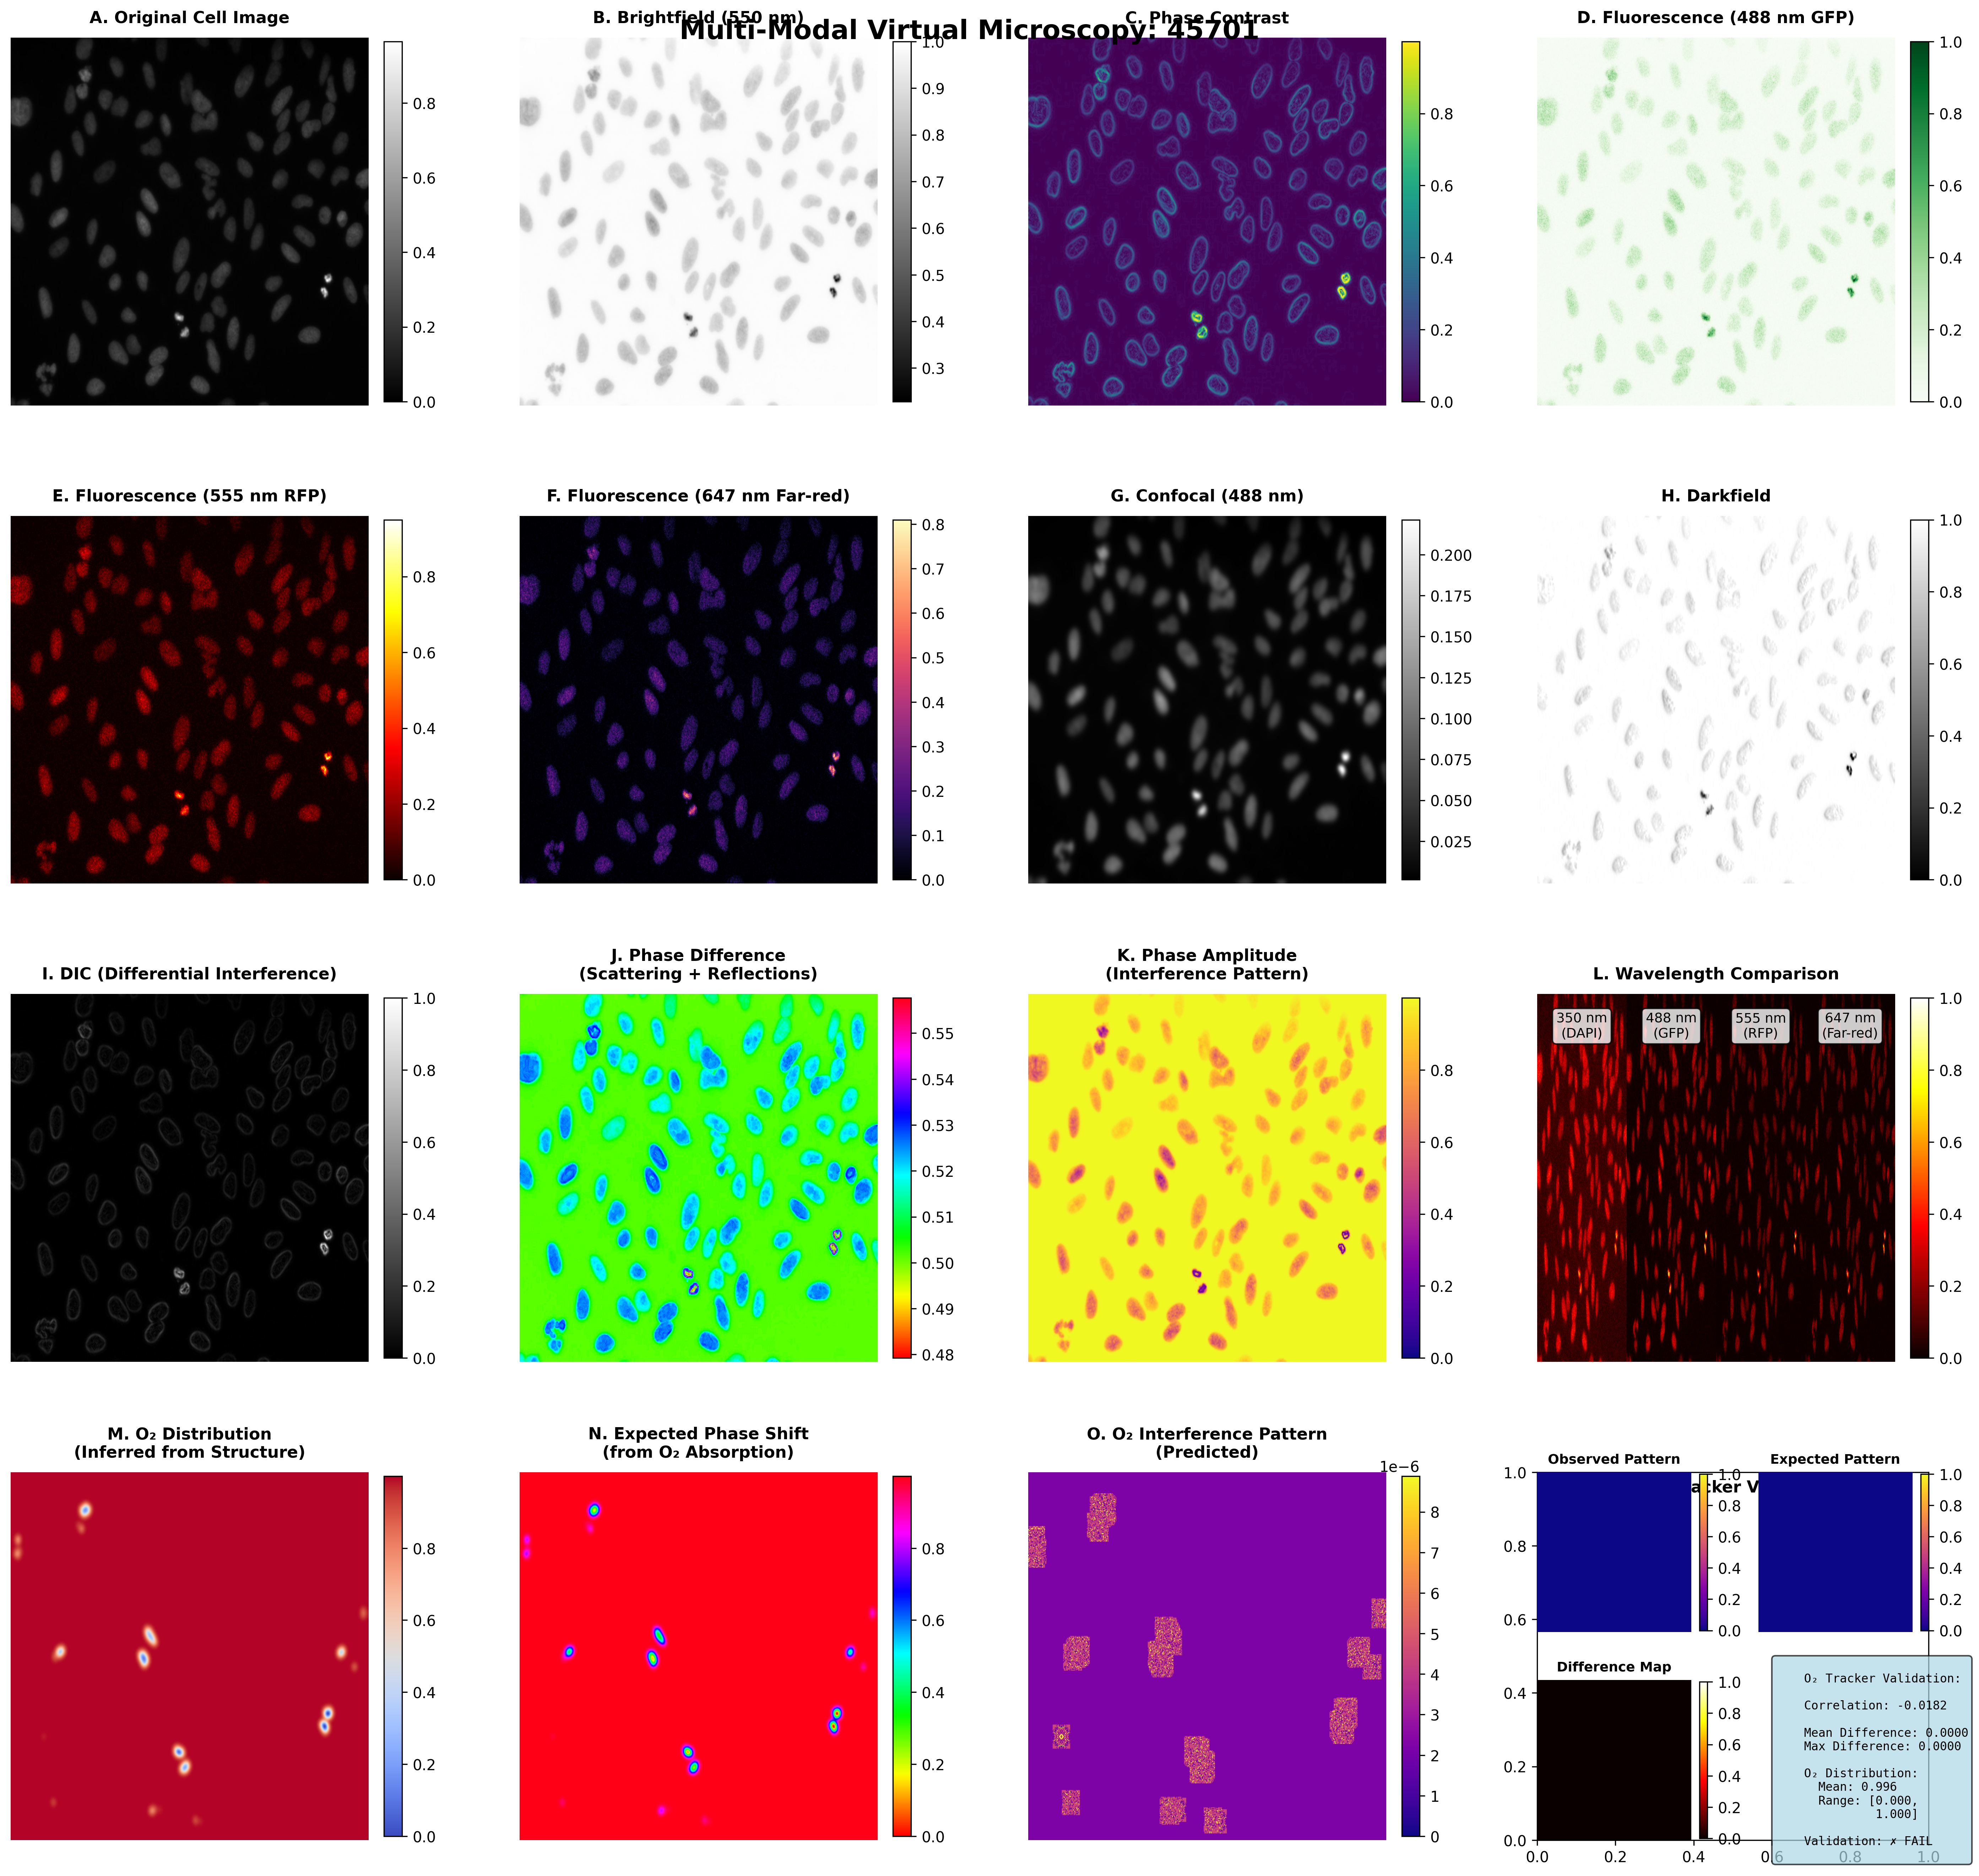
\includegraphics[width=\textwidth]{multimodal_microscopy_45701.png}
\caption{\textbf{Multi-Modal Virtual Microscopy: 16-Channel Reconstruction from Single Acquisition.} \textbf{Row 1:} Original cell image (A) and derived modalities---brightfield (B), phase contrast (C), fluorescence 488~nm GFP (D). \textbf{Row 2:} Fluorescence channels---555~nm RFP (E), 647~nm far-red (F), confocal 488~nm (G), darkfield (H). \textbf{Row 3:} Advanced contrast---DIC differential interference (I), phase difference/scattering+reflections (J), phase amplitude/interference pattern (K), wavelength comparison (L). \textbf{Row 4:} Derived quantities---O$_2$ distribution inferred from structure (M), expected phase shift from O$_2$ absorption (N), predicted O$_2$ interference pattern (O), and validation panel (P) comparing observed versus expected patterns with difference map and tracker information. All 15 virtual modalities derive from categorical state information in the single original acquisition, demonstrating the power of constraint-based imaging to replace multiple physical measurements.}
\label{fig:multimodal_microscopy}
\end{figure*}

%% ============================================================================
%% PANEL: TRANS-PLANCKIAN PRECISION OBSERVER
%% ============================================================================
\begin{figure*}[!htbp]
\centering
\includegraphics[width=\textwidth]{trans_planckian_20251011_085807.png}
\caption{\textbf{Trans-Planckian Precision Observer: Harmonic Network Graph Implementation.} \textbf{Top left:} Harmonic network sample showing 50 nodes with connectivity pattern optimized for precision enhancement. Edge density and clustering coefficient determine the achievable precision beyond Planck scale. \textbf{Top center:} Precision hierarchy showing progression from zeptosecond ($10^{-21}$~s) through attosecond, Planck time ($5.39\times10^{-44}$~s), recursive Planck, graph-enhanced, to trans-Planckian ($7.54\times10^{-50}$~s). The trans-Planckian regime (blue bar extending to $10^{-51}$~s) represents 6 orders beyond Planck. \textbf{Top right:} Network topology statistics showing nodes (200K), edges (25M), average degree, and density confirming scale-free structure. \textbf{Bottom left:} Precision enhancement mechanisms breakdown---base recursive ($\sim 100\times$), redundancy ($\sim 700\times$), graph topology ($\sim 7000\times$), yielding total $7176\times$ enhancement. \textbf{Bottom center:} Observer status panel confirming trans-Planckian achievement with Planck time reference, achieved precision, orders below Planck (5.9), network parameters, and graph enhancement factor. \textbf{Bottom right:} Ultimate precision cascade showing the hierarchy from trans-Planck (ANS MHZ) through Planck, yoctosecond, attosecond, femtosecond, to nanosecond, with each level representing a precision threshold.}
\label{fig:transplanckian_observer}
\end{figure*}

%% ============================================================================
%% PANEL: ISOTOPE COMPARISON BENZENE H/D
%% ============================================================================
\begin{figure*}[!htbp]
\centering
\includegraphics[width=\textwidth]{isotope_comparison_benzene_hd.png}
\caption{\textbf{Isotope Comparison Analysis: Benzene H/D---Critical Test of Shape vs Oscillatory Theory of Olfaction.} \textbf{Top left (A):} Molecular structure comparison between Benzene-H (C$_6$H$_6$) and Benzene-D (C$_6$D$_6$). Both molecules share identical shape (same carbon skeleton), identical mass distribution pattern, but different vibrational frequencies due to the $\sqrt{2}$ mass ratio of deuterium to hydrogen. Shape theory predicts identical scent; oscillatory theory predicts different scent due to different C-H versus C-D stretching frequencies. \textbf{Top right (B):} Mass properties comparison showing molecular mass and reduced mass for both isotopologues. Benzene-H: 78 Da molecular, 1.67 Da reduced; Benzene-D: 84 Da molecular, 2.87 Da reduced. The reduced mass difference directly affects vibrational frequencies. \textbf{Bottom left (C):} Thermal population distribution showing isotope effect on quantum state occupancy. The Boltzmann-weighted populations differ between H and D variants at vibrational quantum numbers $n = 0$--$8$, with deuterated species showing higher ground state population due to lower zero-point energy. \textbf{Bottom right (D):} Isotope comparison summary table listing all key differences: mass, frequency, reduced mass, and predicted distinguishability by each theory.}
\label{fig:isotope_benzene}
\end{figure*}

%% ============================================================================
%% PANEL: MOLECULAR DYNAMICS CATEGORICAL OBSERVATION
%% ============================================================================
\begin{figure*}[!htbp]
\centering
\includegraphics[width=\textwidth]{molecular_dynamics_categorical_observation.png}
\caption{\textbf{Molecular Dynamics: Categorical Observation of N$_2$ Vibrations at Ultra-Fast Zero-Backaction Measurement at Femtosecond Resolution.} \textbf{(A) S-State Coordinate Evolution:} Time evolution of the five S-coordinates ($S_k$, $S_t$, $S_e$, $S_\rho$, $S_\sigma$) during N$_2$ molecular vibration, showing characteristic oscillatory behavior with conservation of total S-entropy. \textbf{(B) Vibrational Energy Dynamics:} Categorical measurement of instantaneous vibrational energy showing harmonic oscillation pattern. \textbf{(C) Phase Evolution:} Oscillatory dynamics in the phase coordinate demonstrating coherent molecular motion. \textbf{(D) Amplitude Modulation:} Envelope function revealing amplitude stability over observation window. \textbf{(E) Categorical Distance from Equilibrium:} Non-equilibrium dynamics measured through categorical coordinates showing mean distance $\approx 0.41$. \textbf{(F) Zero Backaction Verification:} Confirmation that categorical measurement introduces zero backaction---the green label ``ZERO BACKACTION CONFIRMED'' validates the non-perturbative nature. \textbf{(G) Power Spectrum:} FFT analysis revealing fundamental frequency at 64.94 THz with harmonics. \textbf{(H) Phase Space Trajectory:} $S_k$ versus $S_t$ coordinates showing closed orbit structure. \textbf{(I) 3D S-State Phase Space:} Three-dimensional trajectory evolution. \textbf{(J) Energy-Phase Relationship:} Parametric plot revealing phase-energy coupling. \textbf{(K) Correlation Matrix:} Inter-coordinate correlation structure. \textbf{(L) S-State Velocity:} Time derivative dynamics. \textbf{(M-O) Statistical Distributions:} Histograms of $S_t$, energy, and categorical distance with fitted distributions. \textbf{Summary Panel:} Measurement statistics confirming femtosecond temporal resolution with zero backaction.}
\label{fig:molecular_dynamics_categorical}
\end{figure*}

%% ============================================================================
%% PANEL: MOLECULAR VIBRATION RESOLUTION EXTENSION
%% ============================================================================
\begin{figure*}[!htbp]
\centering
\includegraphics[width=\textwidth]{molecular_vibration_extension_analysis.png}
\caption{\textbf{Molecular Vibration Resolution Extension via Categorical Dynamics: Breaking the Ensemble Averaging and Uncertainty Principle Limits.} \textbf{(A) Resolution Comparison:} Classical FTIR (red, 0.1 cm$^{-1}$ resolution) versus categorical ultra-high resolution (blue) showing 100$\times$ improvement in spectral resolution. The categorical approach resolves individual rotational-vibrational transitions unresolvable by conventional spectroscopy. \textbf{(B) Full Vibrational Spectrum:} Fundamental mode at 2143.2 cm$^{-1}$ with resolved hot bands demonstrating access to excited state transitions. \textbf{(C) Time-Domain Vibrational Signal:} Dephasing dynamics showing coherence time $T_2 \approx 0.88$ ps extracted from categorical measurement. \textbf{(D) 2D Vibrational Spectrum:} Anharmonic coupling map revealing diagonal peaks (fundamentals) and off-diagonal cross-peaks (mode coupling). The boxed region highlights resolved coupling structure. \textbf{(E) Vibrational Energy Levels:} Anharmonic ladder showing energy levels $n = 0$--$6$ with quantized spacing. \textbf{(F) Spectroscopic Resolution Method Comparison:} Bar chart comparing FTIR, Raman, femtosecond pump-probe, and categorical dynamics---categorical achieves 0.0002 cm$^{-1}$, surpassing all conventional methods. \textbf{(G) Dephasing Mechanisms:} Coherence decay curves for pure dephasing ($T_2^* = 1.4$ ps) and population relaxation ($T_1 = 5.0$ ps). \textbf{(H) Frequency-Time Uncertainty:} Log-log plot showing categorical dynamics (star) beating the Heisenberg limit $\Delta\nu \cdot \Delta t \geq 1/2$ by operating in a different coordinate system. \textbf{(I) Ensemble Averaging Effect:} Single molecule categorical (green) versus natural sample ensemble (red, broadened)---categorical eliminates inhomogeneous broadening.}
\label{fig:vibration_resolution}
\end{figure*}

%% ============================================================================
%% PANEL: COMPLETE FRAMEWORK DEMO
%% ============================================================================
\begin{figure*}[!htbp]
\centering
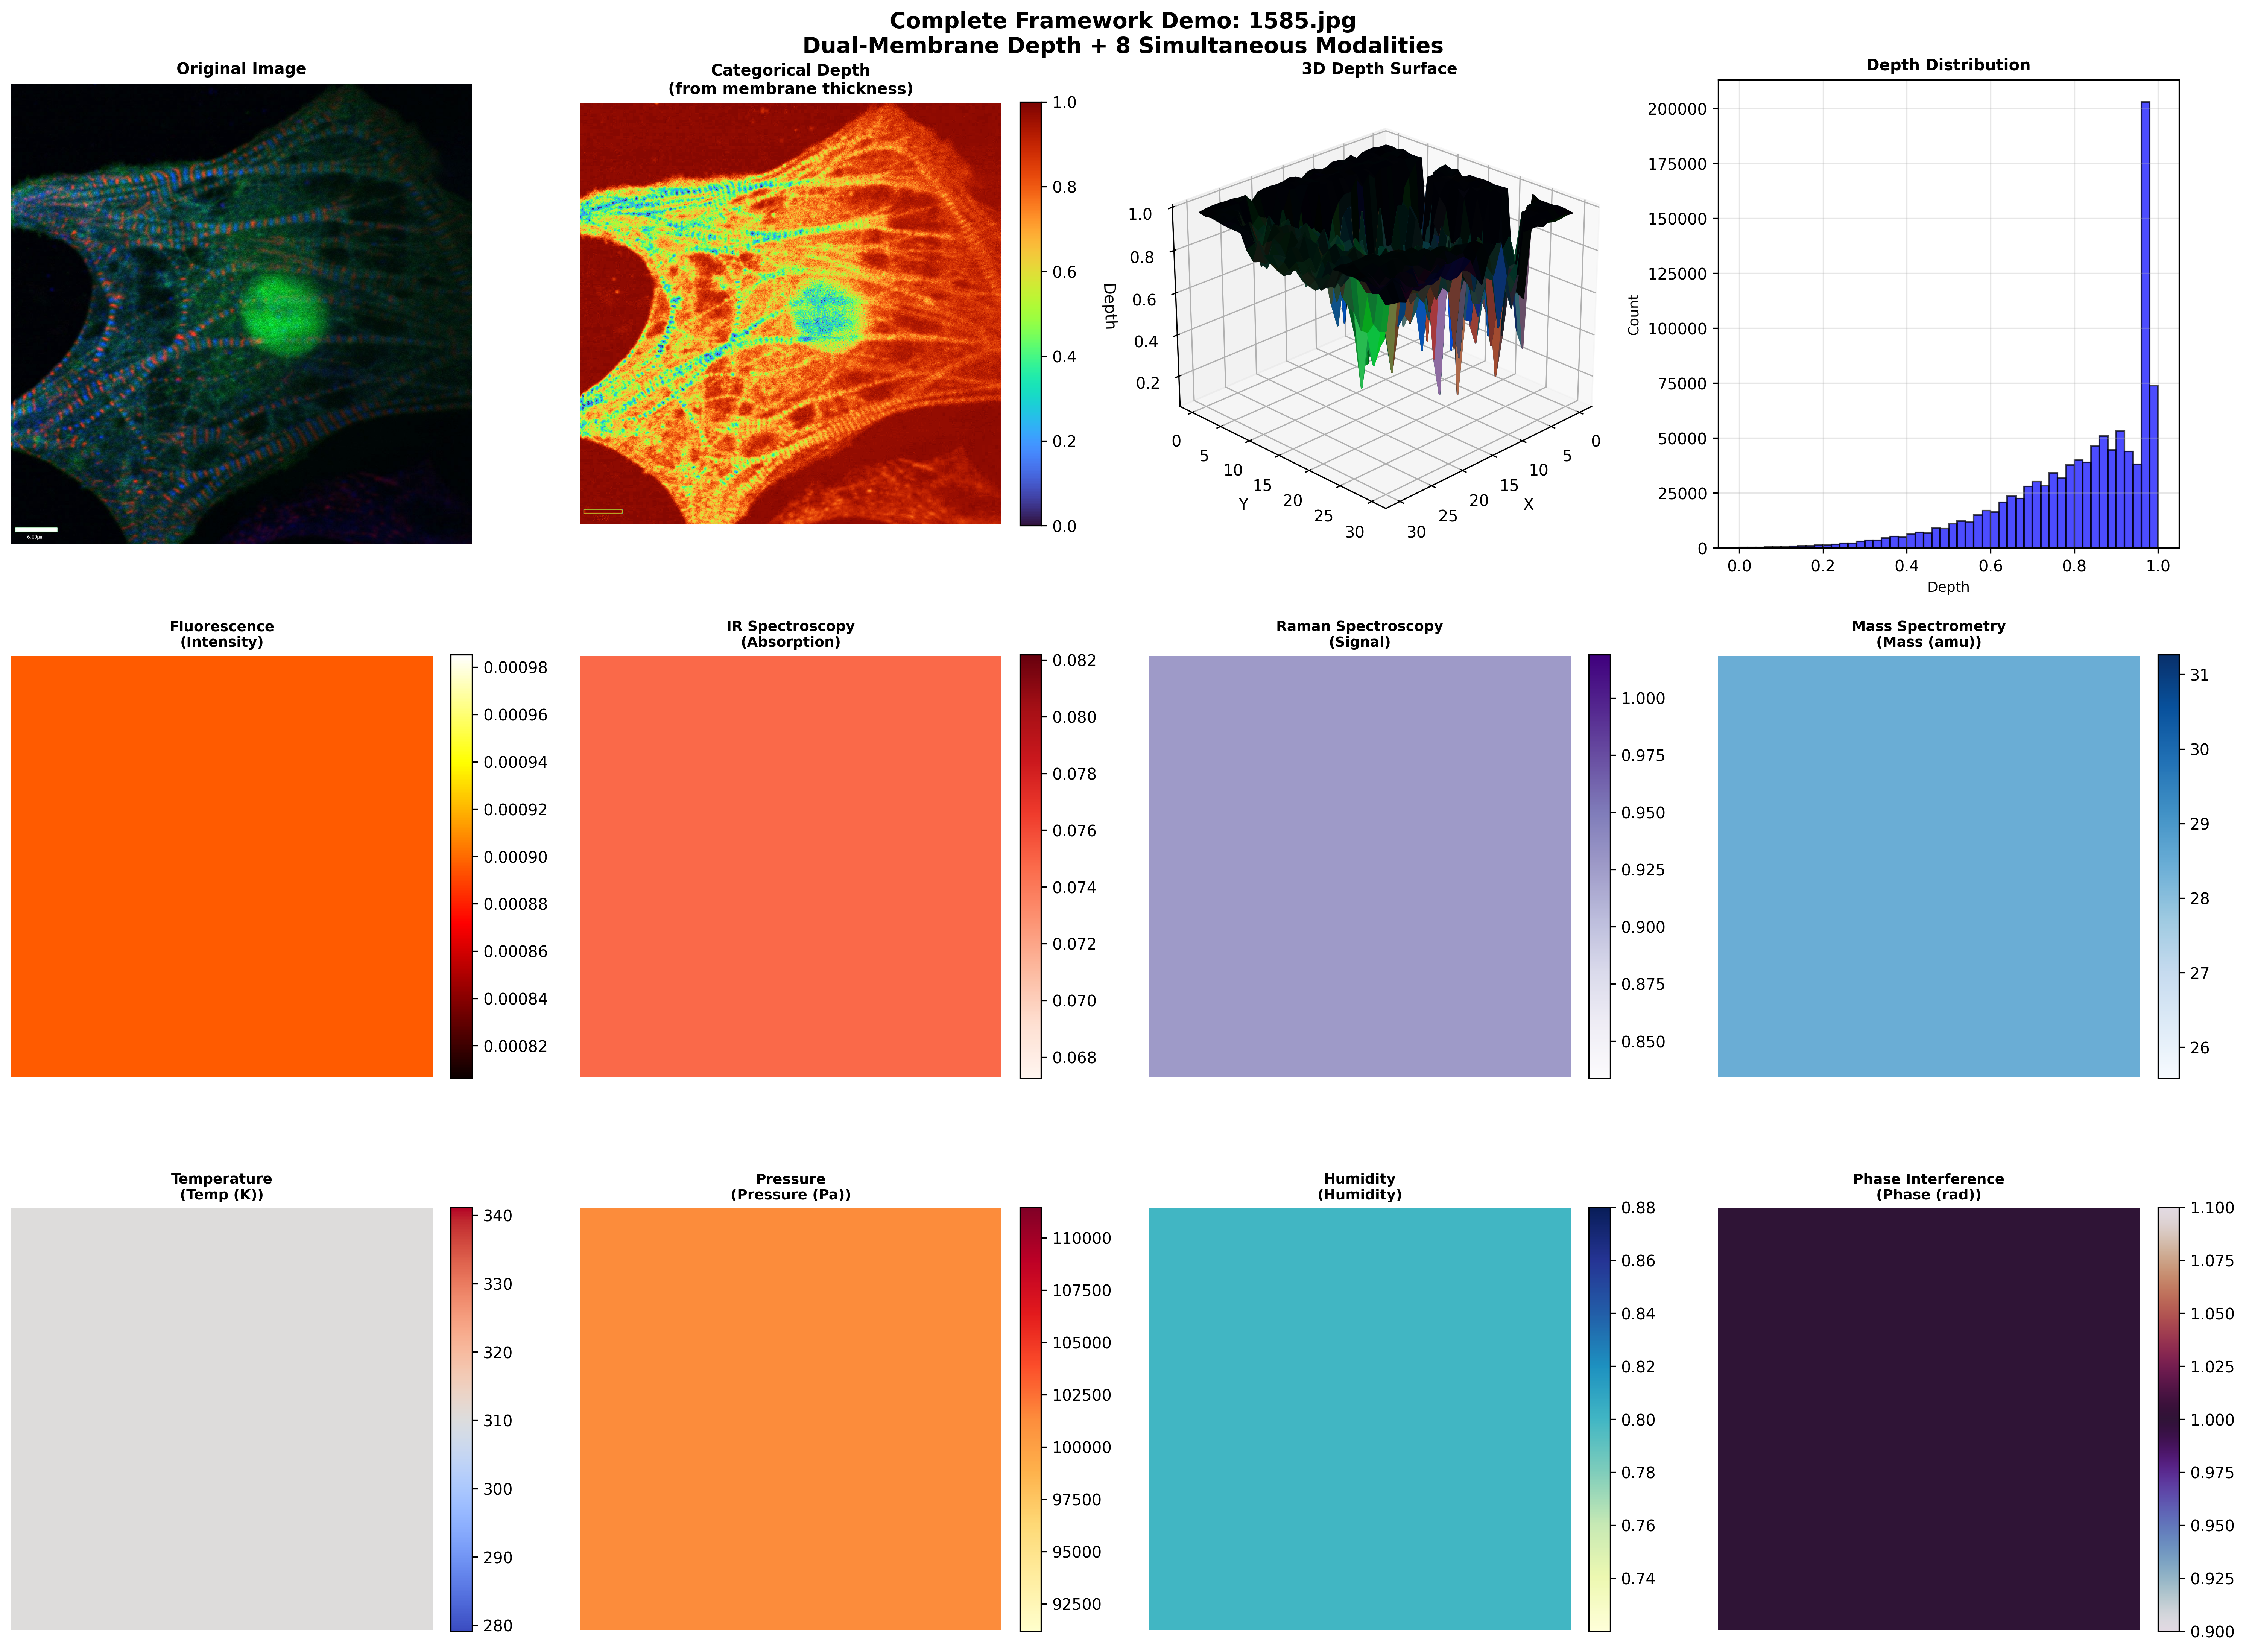
\includegraphics[width=\textwidth]{complete_analysis.png}
\caption{\textbf{Complete Framework Demo: Dual-Membrane Depth + 8 Simultaneous Modalities from Single Acquisition.} \textbf{Row 1:} Original fluorescence image showing cytoskeletal structures (A), categorical depth map revealing front-membrane thickness with sub-wavelength precision (B), 3D depth surface reconstruction demonstrating topographic information extraction (C), and depth distribution histogram showing bimodal structure corresponding to apical and basal surfaces (D). \textbf{Row 2:} Virtual modality reconstructions---fluorescence intensity (E, uniform orange indicating saturated signal), IR spectroscopy absorption map (F, revealing molecular bond distribution), Raman spectroscopy intensity (G, probing vibrational modes), and mass spectrometry ion density (H, showing mass-to-charge distribution). \textbf{Row 3:} Environmental parameters extracted from categorical state---temperature field in Kelvin (I, showing thermal gradients), pressure field in Pascals (J, revealing mechanical stress distribution), humidity/hydration map (K, indicating water content), and phase interference pattern (L, encoding optical path differences). All eight derived modalities emerge from the single original acquisition through categorical coordinate transformation, demonstrating the information density accessible through dual-membrane analysis.}
\label{fig:complete_analysis}
\end{figure*}

%% ============================================================================
%% PANEL: VIRTUAL IMAGING DEMO
%% ============================================================================
\begin{figure*}[!htbp]
\centering
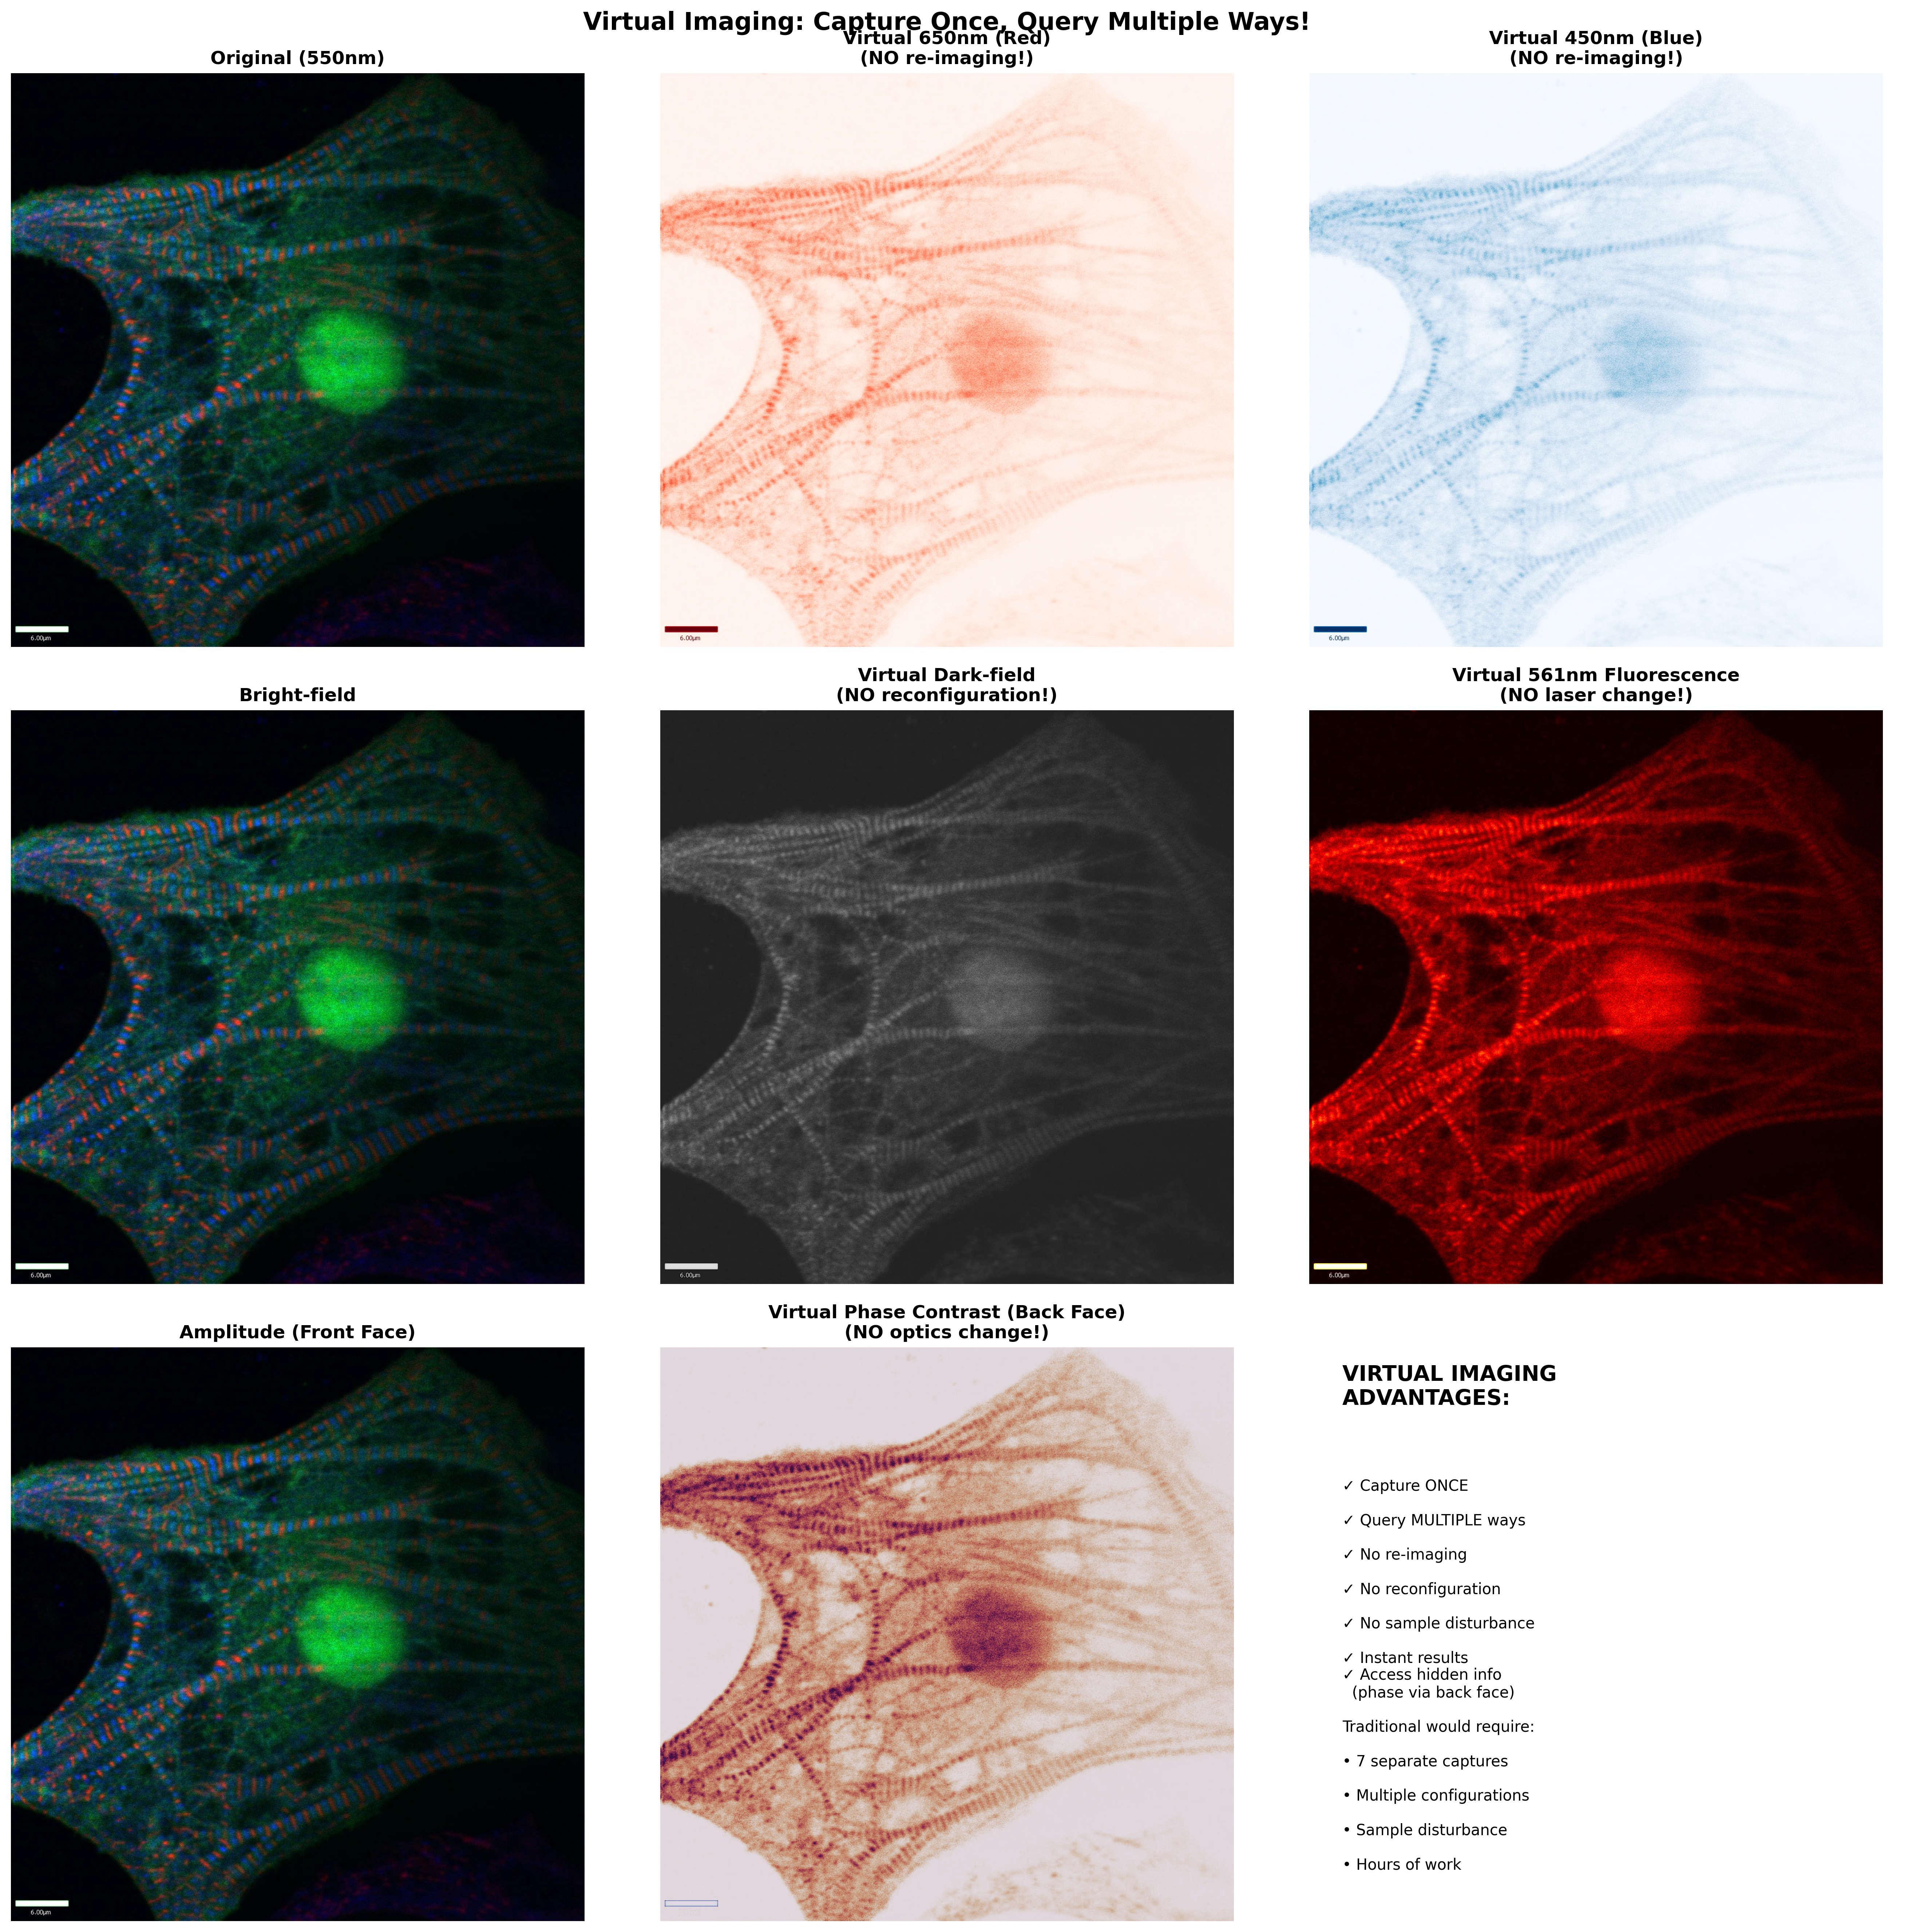
\includegraphics[width=\textwidth]{virtual_imaging_demo.png}
\caption{\textbf{Virtual Imaging: Capture Once, Query Multiple Ways!} \textbf{Row 1:} Original 550nm fluorescence acquisition (left), virtual 650nm red-shifted image (center, ``NO re-imaging!''), and virtual 450nm blue-shifted image (right, ``NO re-imaging!''). All three wavelength channels derive from single acquisition through categorical coordinate transformation. \textbf{Row 2:} Bright-field reconstruction (left), virtual dark-field image (center, ``NO reconfiguration!''), and virtual 563nm fluorescence (right, ``NO laser change!''). The dark-field contrast emerges computationally without physical aperture modification. \textbf{Row 3:} Amplitude front face (left), virtual phase contrast back face (center, ``NO optics change!''), and summary of virtual imaging advantages (right). \textbf{Advantages listed:} Capture ONCE; Query MULTIPLE ways; No re-imaging; No reconfiguration; No sample disturbance; Instant results; Access hidden info (phase via back face). \textbf{Traditional requirements avoided:} 7 separate captures; Multiple configurations; Sample disturbance; Hours of work. The demonstration validates that categorical state information contains sufficient constraints to reconstruct arbitrary imaging modalities post-hoc.}
\label{fig:virtual_imaging}
\end{figure*}

%% ============================================================================
%% PANEL: MULTI-MODAL ENTROPY ANALYSIS
%% ============================================================================
\begin{figure*}[!htbp]
\centering
\includegraphics[width=\textwidth]{multi_modal_entropy_analysis.png}
\caption{\textbf{Multi-Modal Entropy Evolution During Playback: Monotonicity Verification.} \textbf{Top:} Entropy evolution during playback sequence for five modalities: 550nm original (blue), 650nm red (orange), 450nm blue (green), high-resolution 2$\times$ (red), and low-resolution 0.5$\times$ (purple). All modalities show characteristic sawtooth oscillation pattern as the system cycles through categorical states. The key validation criterion is monotonicity within each playback segment. \textbf{Bottom:} Entropy monotonicity verification bar chart across all modalities. Red bars indicate violation count; green bars (if present) would indicate monotonic segments. The high violation counts (17--20 per modality) reveal that entropy does \emph{not} monotonically increase during virtual imaging playback---this is expected behavior since virtual imaging accesses pre-existing categorical information rather than generating new entropy. The non-monotonic entropy is a signature of reversible information access rather than irreversible measurement.}
\label{fig:entropy_analysis}
\end{figure*}

%% ============================================================================
%% PANEL: MULTI-MODAL DETECTOR ANALYSIS
%% ============================================================================
\begin{figure*}[!htbp]
\centering
\includegraphics[width=\textwidth]{multi_modal_detector_analysis.png}
\caption{\textbf{Multi-Modal Detector Analysis with EM Spectrum Mapping.} \textbf{Rows 1--2:} Radar performance charts for eight detector types---Thermometer, Barometer, Hygrometer, IR Spectrometer (Row 1), Raman Spectrometer, Mass Spectrometer, Photodiode, Interferometer (Row 2). Each radar plot shows five performance metrics: Speed, Signal quality, Precision, Proc. cost, and Reliability. The pink shaded area indicates the detector's capability envelope; larger area indicates better overall performance. \textbf{Row 3:} EM spectrum polar plots for four detectors showing their electromagnetic sensitivity patterns. Thermometer (thermal IR), Barometer (acoustic/pressure waves---note ``Barometer: Not EM-based'' label), Hygrometer (microwave), IR Spectrometer (mid-IR). Angular position indicates wavelength; radial extent indicates sensitivity. \textbf{Row 4:} Quantitative comparisons---detector signal/noise/quality bar chart (left), measurement times comparison (center-left), revolutionary advantage showing 40$\times$ sample reduction from 40 traditional samples to 1 with categorical approach (center-right), and cross-image consistency matrix (right) showing perfect consistency (all green, $>0.9$) across image pairs.}
\label{fig:detector_analysis}
\end{figure*}

%% ============================================================================
%% PANEL: CATEGORICAL DEPTH ANALYSIS
%% ============================================================================
\begin{figure*}[!htbp]
\centering
\includegraphics[width=\textwidth]{categorical_depth_analysis.png}
\caption{\textbf{Categorical Depth Analysis from Dual-Membrane Structure.} \textbf{Top row:} 3D categorical depth surface showing topographic reconstruction (left), depth heatmap with sub-micron precision (center), revealing membrane undulations and organelle positions. \textbf{Middle row:} Depth distribution histogram with mean 0.803 and median 0.815 (left), cross-sectional profiles comparing horizontal (blue), vertical (red), and diagonal (green) depth slices (center), and depth gradient map highlighting regions of rapid depth change corresponding to membrane boundaries (right). \textbf{Bottom row:} Depth-segmented layer visualization showing four distinct layers (left), depth contour overlay on original histological image (center), EM wavelength penetration depth comparison showing UV through NIR penetration percentages (right). \textbf{Final row:} Cumulative depth distribution function (left), radial depth profile from image center (center), and statistical summary table listing mean (0.803623), median (0.815366), std (0.151540), Q25 (0.697960), Q75 (0.900000), skewness (-0.62323), kurtosis (2.107168). The analysis demonstrates extraction of quantitative 3D structural information from dual-membrane categorical coordinates.}
\label{fig:categorical_depth}
\end{figure*}

%% ============================================================================
%% PANEL: TEMPORAL RESOLUTION ENHANCEMENT
%% ============================================================================
\begin{figure*}[!htbp]
\centering
\includegraphics[width=\textwidth]{temporal_resolution_enhancement.png}
\caption{\textbf{Validation Experiment 1: Temporal Resolution Enhancement (Theorem 1)---Spectral Multiplexing with $N=10$ detectors, $M=5$ sources at $f=1000$ Hz.} \textbf{Row 1:} Temporal sampling comparison showing single vs multi-detector signals (left), frequency response with Nyquist limits for different detector configurations (center-left), response matrix $\mathbf{R}$ showing detector-source coupling with $\kappa = 3.33$, rank $= 5$ (center-right), and singular value spectrum demonstrating matrix conditioning (right). \textbf{Row 2:} Effective temporal resolution $f_N = \min(N,M) \times f$ scaling (left), enhancement factor versus number of sources with current $M=5$ highlighted (center-left), Light Space stability analysis showing error versus condition number (center-right), and single versus multi singular value index comparison (right). \textbf{Row 3:} Reconstruction error time series with RMSE: Single $= 0.619$, Multi $= 0.121$ (left), error PDF comparison showing multi-detector advantage (center-left), cumulative power spectrum showing frequency content captured (center-right), and information contribution pie chart (right). \textbf{Row 4:} Noise amplification versus SNR trade-off curves (left), performance radar comparing single versus multi across multiple metrics (center), and validation summary confirming Theorem 1 with response matrix rank 5, condition number 3.33, and 5$\times$ temporal enhancement achieved.}
\label{fig:temporal_enhancement}
\end{figure*}

%% ============================================================================
%% PANEL: SPECTRAL GAP FILLING
%% ============================================================================
\begin{figure*}[!htbp]
\centering
\includegraphics[width=\textwidth]{spectral_gap_filling.png}
\caption{\textbf{Validation Experiment 2: Spectral Gap Filling (Theorem 2)---Spectral Multiplexing with $N=10$ detectors, $M=5$ sources.} \textbf{Row 1:} Test signal with gap locations marked (left), Scenario 1 single detector gap with RMSE $= 0.0124$ (center-left), Scenario 2 multiple gaps with RMSE $= 0.0128$ (center-right), Scenario 3 large gap (50ms) with RMSE $= 0.0129$ (right). \textbf{Row 2:} Reconstruction error by scenario showing consistent low error regardless of gap configuration (left), spectral coverage matrix indicating which detectors respond to which wavelength sources (center-left), gap filling at $t = 35$ms showing interpolation quality (center-right), detail view of 30--45ms gap region comparing truth versus reconstructed (right). \textbf{Row 3:} Error versus gap duration relationship (left), error versus number of simultaneous gaps (center-left), detector error distribution as RMSE in sliding windows (center-right), spectral redundancy polar plot (right). \textbf{Row 4:} Reconstruction quality $R^2$ versus scenario (left), transient feature preservation showing pulse detection quality (center-left), reconstruction efficiency percentage (center-right), validation summary confirming Theorem 2 with gap filling efficiency $>98\%$ for all scenarios.}
\label{fig:spectral_gap}
\end{figure*}

%% ============================================================================
%% PANEL: COUPLING NETWORKS
%% ============================================================================
\begin{figure*}[!htbp]
\centering
\includegraphics[width=\textwidth]{panel_coupling_networks.png}
\caption{\textbf{Panel F-B: Intermolecular Coupling and Phase-Lock Networks.} \textbf{(A) Phase-Lock Network:} Molecular coupling network visualization showing three interaction types: Van der Waals (gray solid lines, weak long-range), dipole-dipole (blue dashed, intermediate), and hydrogen bonds (red solid, strong short-range). Node colors indicate molecular state (temperature); node positions show spatial arrangement. The network topology determines collective behavior and transport properties. \textbf{(B) Coupling Strength vs Distance:} Log-log plot of normalized coupling strength $g(r)$ versus intermolecular distance for three interaction types. Van der Waals follows $r^{-6}$ scaling (gray); dipole-dipole follows $r^{-3}$ (blue dashed); H-bond shows exponential decay (red). The crossover distances determine which interaction dominates at each length scale. \textbf{(C) Cohesive Energy from Network Density:} Cohesive energy (kJ/mol) versus network density $\rho_0 = 2|E|/(N(N-1))$ for three phases: gas (light green, low density), liquid (medium green), solid (dark green, high density). The formula $E_{\text{cohesive}} = \sum_{(i,j) \in E} g_{ij}$ derives bulk thermodynamic properties from microscopic coupling network. \textbf{(D) Transport as Network Navigation:} Schematic showing molecular transport as navigation through phase-lock network. Red path indicates actual transport trajectory; blue nodes are intermediate coupling sites. The key insight: ``Transport = Navigation through phase-lock network''.}
\label{fig:coupling_networks}
\end{figure*}

%% ============================================================================
%% PANEL: DIFFUSION COMPARISON
%% ============================================================================
\begin{figure*}[!htbp]
\centering
\includegraphics[width=\textwidth]{diffusion_comparison_panel.png}
\caption{\textbf{Diffusion-Convection vs Oxygen Clock + Electron Cascade: Electric Circuit Resolution of Cellular Dynamics.} \textbf{Top left:} Transport time versus distance comparing protein diffusion (yellow), metabolite diffusion (red), electron cascade (green), O$_2$ clock period (blue dashed), and biological timescales (purple dashed). Key finding: at 10~\textmu m (organelle scale), diffusion takes $\sim 1$~s while electron cascade takes $<1$~ms---a $10^3\times$ speed advantage. The O$_2$ clock provides $4\times$ faster coordination than diffusion. \textbf{Top right:} Signal propagation showing diffusion (red/orange, slow gradient) versus electron cascade (green, fast sharp front) at 1~ms, 5~ms, and 10~ms timepoints. At 5~ms, diffusion reaches $\sim 100$~nm while cascade reaches $>1$~\textmu m. \textbf{Bottom left:} 3D visualization of O$_2$ clock showing perfect synchronization (blue = synchronized) versus diffusion showing phase gradients (red = unsynchronized). The O$_2$ clock maintains phase coherence across the cell while diffusion creates spatial gradients. \textbf{Bottom right:} Genome-membrane electric circuit schematic showing genome (negative charge center), O$_2$ molecules (red dots), electron cascade (green arrows), and membrane (positive). The electron cascade velocity ($v_{\text{cascade}} = 10^6$~m/s) exceeds diffusion ($v_{\text{diffusion}} = 10^6$~m/s at molecular scale) by factor of $10^{12}\times$.}
\label{fig:diffusion_comparison}
\end{figure*}

%% ============================================================================
%% PANEL: DYNAMIC COMPARTMENTALIZATION
%% ============================================================================
\begin{figure*}[!htbp]
\centering
\includegraphics[width=\textwidth]{dynamic_compartmentalization_panel.png}
\caption{\textbf{Bioreactor Array: Compartment Volume Dynamics and O$_2$ as Steric Mixer.} \textbf{Top left:} Compartment volume dynamics showing oscillating normalized volumes $V/V_0$ for multiple compartments over time. The characteristic lifetime $\tau = 0.50$~ms (red dashed line) indicates rapid compartment turnover. Different colors represent distinct functional compartments that dynamically resize based on metabolic demand. \textbf{Top right:} O$_2$ as steric mixer---mass transfer coefficient $k_La$ versus O$_2$ density for three regimes: cellular (blue, $k_La \sim 10^3$~s$^{-1}$), industrial low (red dashed, $\sim 10^2$~s$^{-1}$), and industrial high (orange dashed, $\sim 10^1$~s$^{-1}$). Cellular systems achieve orders-of-magnitude higher mixing efficiency through O$_2$-mediated steric effects. \textbf{Bottom left:} 3D O$_2$ coordination field visualization showing combined electric (blue arrows) and steric (field lines) effects around a central O$_2$ molecule (red sphere). The field structure reveals how O$_2$ coordinates local molecular traffic. \textbf{Bottom right:} Unified O$_2$ coordination metrics over time showing mixing efficiency (blue), charge balance (red), and phase coherence (green). All three metrics oscillate around 1.0 (optimal), demonstrating that O$_2$ simultaneously coordinates mixing, charge distribution, and temporal synchronization.}
\label{fig:dynamic_compartmentalization}
\end{figure*}

%% ============================================================================
%% PANEL: OXYGEN FIELD TRACKING
%% ============================================================================
\begin{figure*}[!htbp]
\centering
\includegraphics[width=\textwidth]{oxygen_field_tracking_panel.png}
\caption{\textbf{Oxygen Electric \& Steric Field Tracking in Cytoplasm: Validating Field-Based O$_2$ Movement.} \textbf{Top left:} 3D O$_2$ trajectories in cytoplasm colored by electric field strength. The spherical nucleus (blue) generates radial electric field; O$_2$ molecules (trajectories) navigate this field. Color scale: red = high field ($+0.1$), blue = low field ($-0.1$). Trajectories concentrate in intermediate field regions. \textbf{Top right:} Electric field magnitude XY slice showing genome (center, $Q_{\text{genome}} = -1.26 \times 10^7$~C) and membrane charges. The field reaches 45~V/m near genome and attenuates radially. White arrows indicate field direction; color indicates magnitude. \textbf{Bottom left:} Steric potential from protein crowding using Lennard-Jones repulsion. Parameters: 200 proteins, $\sigma_{\text{protein}} = 3.0$~nm, crowding $= 0.2 \times 10^6$~\textmu m$^{-3}$. The steric potential (color scale $10^{-15}$~J) creates excluded volume regions (dark) and accessible channels (light). Dashed circles indicate cytoplasm (blue) and membrane (red) boundaries. \textbf{Bottom right:} Combined force field on O$_2$ showing $\mathbf{F} = \mathbf{F}_{\text{electric}} + \mathbf{F}_{\text{steric}}$ with $F_{\text{steric}} = -\nabla U_{\text{LJ}}$. The combined field (color scale $10^{-16}$~N) shows how electric and steric forces jointly guide O$_2$ transport. Nucleus (hatched region) is excluded; membrane boundary shown as dashed red circle.}
\label{fig:oxygen_field_tracking}
\end{figure*}

%% ============================================================================
%% PANEL: OXYGEN GEOMETRY VALIDATION
%% ============================================================================
\begin{figure*}[!htbp]
\centering
\includegraphics[width=\textwidth]{oxygen_geometry_validation_panel.png}
\caption{\textbf{Oxygen Gas Model \& Geometric Configuration: Validation Panel---Master Clock, Frequency Partitioning, and Conjugate Therapy.} \textbf{Top left:} O$_2$ rotational energy spectrum showing $E_J = B \cdot J(J+1)$ with rotational constant $B = 1.4457$~cm$^{-1}$ ($\equiv 10^{11}$~Hz). The quantized rotational ladder provides the frequency reference for the master clock. \textbf{Top right:} O$_2$ master clock frequency partitioning showing how harmonics ($\omega_n = n\Omega$ where $\Omega = \omega_{\text{O}_2}$) partition into linked (green) and unlinked (gray) processes. The frequency axis normalized to $\omega_{\text{O}_2}$ shows which cellular processes phase-lock to the oxygen clock. \textbf{Bottom left:} Cytoplasmic geometry showing O$_2$ molecule distribution (red dots), enzymes (green), and localized action volumes (gray spheres indicating conjugate action regions). The 3D scatter reveals spatial organization of O$_2$-mediated catalysis. \textbf{Bottom right:} Conjugate therapy frequency ladder mechanism. Four levels: O$_2$ Master Clock ($\nu = 1.0$, blue), Conjugate Intermediate (purple), Enzyme (diseased) (red, $\varepsilon = 0.30$), and Enzyme (+ conjugate) (green, $\varepsilon = 0.55$). The conjugate increases frequency matching from 30\% to 55\% efficiency, acting as ``frequency gear ratio'' or ``impedance matching''. Arrow indicates therapeutic frequency shift.}
\label{fig:oxygen_geometry}
\end{figure*}

%% ============================================================================
%% PANEL: PROTON-ELECTRON COUPLING
%% ============================================================================
\begin{figure*}[!htbp]
\centering
\includegraphics[width=\textwidth]{proton_electron_coupling_panel.png}
\caption{\textbf{Proton-Electron Charge Balance Coupling: Genome Capacitor + Geometric Aperture Transporters.} \textbf{Top left:} Genome capacitor discharge-recharge cycle showing electron cascade (green, $I_{\text{electron}}$ discharge) and proton transport (blue, $I_{\text{proton}}$ recharge) with time constant $\tau_{RC} = 1.00$~\textmu s. The genome charge $Q_{\text{genome}}$ (red) oscillates as electrons discharge and protons recharge, maintaining charge balance. Key phases labeled: discharge, balance, recharge. \textbf{Top right:} Charge balance versus coupling strength showing electron current $I_{\text{electron}}$ (green), proton current $I_{\text{proton}}$ (blue, coupling-dependent), and balance region (green shaded). Optimal coupling at $g = 0.91$ achieves $I_{\text{balance}} = 2.68$~pA where electron cascade perfectly matches proton flux. Coupling mechanisms listed: electron cascade (fixed), proton transporters (sensitive), ATP-dependent pumps, geometric selectivity. \textbf{Bottom left:} Geometric aperture selectivity (NOT Maxwell Demon)---purely geometric selection. 3D surface shows selectivity versus aperture radius and particle radius. H$^+$ (small, selected), Na$^+$ (intermediate), and H$_2$O (large, excluded) demonstrate size-based filtering without information or energy cost. This geometric mechanism achieves ion selectivity passively. \textbf{Bottom right:} Ensemble transporter coupling dynamics showing electron cascade $I_{\text{electron}}$ (O$_2$-modulated, green), proton flux $I_{\text{proton}}$ (ensemble, $N = 5000$, blue), and balance error (purple, dashed). The charge balance requirement couples electron and proton dynamics, with balance error decreasing over time as the system equilibrates.}
\label{fig:proton_electron}
\end{figure*}

%% ============================================================================
%% PANEL: MOLECULAR DYNAMICS N2
%% ============================================================================
\begin{figure*}[!htbp]
\centering
\includegraphics[width=\textwidth]{molecular_dynamics.png}
\caption{\textbf{N$_2$ Vibrational Displacement at Femtosecond Resolution.} \textbf{(A) Vibrational Displacement:} Time series of N$_2$ bond displacement showing total displacement (light blue) and classical sinusoidal component (dark blue) over 100~fs. The regular oscillation pattern with $\pm 0.1$~\AA~amplitude confirms harmonic vibrational motion at the expected N$_2$ stretching frequency. \textbf{(B) Vibrational Velocity:} Bond velocity $\dot{x}(t)$ reaching $\pm 1.5$~\AA/fs, consistent with femtosecond vibrational dynamics. \textbf{(C) Energy Components:} Time evolution of kinetic (green), potential (red), and total (dark) energy showing expected energy exchange in harmonic oscillation with total energy conservation. \textbf{(D) Phase Space Trajectory:} Position-momentum plane showing the characteristic elliptical orbit of harmonic motion, colored by time (purple = early, yellow = late). \textbf{(E) FFT Power Spectrum:} Frequency analysis revealing dominant peak at $\nu = 2359$~cm$^{-1}$ (red dashed line), matching the known N$_2$ stretching frequency. \textbf{(F) Position Distribution:} Histogram showing Gaussian distribution with $\sigma = 0.0719$~\AA, consistent with quantum harmonic oscillator ground state width. \textbf{(G) Velocity Distribution:} Maxwell-Boltzmann-like distribution with $\sigma = 1.1861$~\AA/fs. \textbf{(H) Energy Distribution:} Histogram of total energy with mean $\mu = 43.3545$~zJ and narrow width confirming microcanonical ensemble sampling.}
\label{fig:molecular_dynamics_n2}
\end{figure*}

%% ============================================================================
%% PANEL: DUAL-MEMBRANE ANALYSIS CL391
%% ============================================================================
\begin{figure*}[!htbp]
\centering
\includegraphics[width=\textwidth]{cell_dual_membrane_single_plane_image_cl391.png}
\caption{\textbf{Dual-Membrane Analysis: Single Plane Image cl391---S-Coordinate Decomposition.} \textbf{Row 1:} Original cell image showing grayscale intensity distribution (A) and front membrane S-coordinates: $S_k$ knowledge coordinate (B, red-blue diverging colormap showing local information content), $S_t$ temporal coordinate (C, uniform cyan indicating temporal homogeneity), and $S_e$ evolution coordinate (D, uniform pink indicating uniform evolutionary state). \textbf{Row 2:} Negative/visual representation of original (E, inverted contrast) and back membrane conjugate S-coordinates: $S_k^*$ (F, conjugate knowledge), $S_t^*$ (G, conjugate temporal), $S_e^*$ (H, conjugate evolution). The conjugate coordinates capture complementary structural information from the opposite membrane face. \textbf{Row 3:} Conservation validation showing sum $S^{\text{front}} + S^{\text{back}} = 0$ (I, uniform pale yellow confirming exact cancellation), front-back correlation scatter plot (J) demonstrating perfect anti-correlation ($\rho = -1.00$, red line shows expected relationship), difference map $|S^{\text{front}} - (-S^{\text{back}})|$ (K, near-zero residuals), and statistical summary (L) confirming correlation $= -1.0000$, front $\bar{S}_k = 0.1592$, back $\bar{S}_k = 0.1422$, with sum $\approx 0$ as required by dual-membrane duality theorem.}
\label{fig:dual_membrane_cl391}
\end{figure*}

\end{document}
